\documentclass[12pt, a4paper]{article}

\title{Physics 2}
\date{} 

% This first part of the file is called the PREAMBLE. It includes
% customizations and command definitions. The preamble is everything
% between \documentclass and \begin{document}.
	
	\usepackage[margin=1in]{geometry}  % set the margins to 1in on all sides
	\usepackage{graphicx}              % to include figures
	\usepackage{amsmath}               % great math stuff
	\usepackage{amsfonts}              % for blackboard bold, etc
	\usepackage{amsthm}                % better theorem environments
	\usepackage{amssymb}               % math symbols
	\usepackage{wrapfig}			   % for images formatting
	\usepackage{booktabs}
	\usepackage{caption}			   % for labeling images
	\usepackage{bigints}			   % for bigger integral symbols	
	\usepackage{subcaption}			   % subfigures functions
%	\usepackage{subfig}				   % subfigures
	\usepackage[many]{tcolorbox}       % For highlighting equations
	\usepackage{circuitikz}			   % for resistor and similar symbols
	\usepackage{mathrsfs}			   % math letters
	\usepackage{tabularx}


	% Fancy E for emf ℰ
	\DeclareFontFamily{U}{calligra}{}
	\DeclareFontShape{U}{calligra}{m}{n}{<->callig15}{}
	
	\newcommand{\calE}{{\!\!\text{\usefont{U}{calligra}{m}{n}E}\,\,}}
	%%%%

	% various theorems, numbered by section
	
	\newtheorem{thm}{Theorem}[section]
	\newtheorem{lem}[thm]{Lemma}
	\newtheorem{prop}[thm]{Proposition}
	\newtheorem{cor}[thm]{Corollary}
	\newtheorem{conj}[thm]{Conjecture}
	
	\DeclareMathOperator{\id}{id}
	
	\newcommand{\bd}[1]{\mathbf{#1}}  % for bolding symbols
	\newcommand{\RR}{\mathbb{R}}      % for Real numbers
	\newcommand{\ZZ}{\mathbb{Z}}      % for Integers
	\newcommand{\col}[1]{\left[\begin{matrix} #1 \end{matrix} \right]}
	\newcommand{\comb}[2]{\binom{#1^2 + #2^2}{#1+#2}}

	\begin{document}
	
		\section*{1. Coulomb's Law}
		
		\textbf{Coulomb's Law} describes the force between two charged particles. If the charges have the same sign, they repel, if they are opposite, they attract. The \textbf{electrostatic force} is given by:
		
		\begin{equation}
			\vec{F} = k \frac{q_1 q_2}{r^2} \hat{r} \tag{Coulomb's Law, 1-1}
		\end{equation}
		
		where:
		\begin{itemize}
			\item $\vec{F}$ is the force,
			\item $q_1$ and $q_2$ are the charges,
			\item $r$ is the distance between them,
			\item $k$ is a constant (\textbf{electrostatic constant}),
			\item $\hat{r}$ is a unit vector along the line connecting the charges.
		\end{itemize}
		
		Coulomb's Law is similar to \textbf{Newton's Law of Gravitation}, which gives the gravitational force between two masses as:
		
		\begin{equation}
			\vec{F} = G \frac{m_1 m_2}{r^2} \hat{r} \tag{Newton's Law of Gravitation, 1-2}
		\end{equation}
		
		Both laws follow an inverse-square relationship, meaning the force decreases with the square of the distance between the objects. However, unlike gravitational forces (which are always attractive), electrostatic forces can be either attractive or repulsive depending on the charges.
		
		Coulomb's law has been experimentally validated and works even at the atomic level, explaining the forces between atomic nuclei and electrons. It also accounts for the forces that bind atoms and molecules together.
		
		In the \textbf{SI unit system}, the unit of charge is the \textit{coulomb} (C), and \textbf{electric current} $i$ is defined as the rate at which charge flows:
		
		\begin{equation}
			i = \frac{dq}{dt} \tag{Electric Current, 1-3}
		\end{equation}
		where $i$ is the current (in ampères) and $dq$ is the charge (in coulombs) passing through a point in time $dt$.
		Rearranging in \textbf{SI} tells us that: 
		
		\begin{equation*}
			1 \, C = (1 \, A)(1 \, s)
		\end{equation*}
		For historical reasons the constant $k$ is usually written as $1/4\pi\varepsilon_0$, therefore the magnitude in Coulomb's Law becomes
		
		\begin{equation}
			\textbf{F} = \frac{1}{4\pi\varepsilon_0} \frac{|q_1||q_2|}{r^2} \tag{Coulomb's Law, 1-4}
		\end{equation}
		The constants in Eqs. 1.1 and 1.4 have values:
		\begin{equation*}
			k = \frac{1}{4\pi\varepsilon_0} = 8.99 \cdot 10^9  \frac{N\cdot m^2}{C^2} 
		\end{equation*}
		The quantity $\varepsilon_0$ is called \textbf{permittivity constant of free space}:
		\begin{equation*}
			\varepsilon_0 = 8.85 \cdot 10^{-12} \frac{C^2}{N\cdot m^2}
		\end{equation*}
		Another parallel between the gravitational force and the electrostatic force is that they both obey the principle of superposition. Given $n$ charged particles we can say that the net force is given by the vector sum:
		\begin{equation*}
			\vec{F_{1,net}} = \vec{F_{1,2}} + \vec{F_{1,3}} + \vec{F_{1,4}} + ... + \vec{F_{1,n}} \tag{1-5}
		\end{equation*}
		
		\subsection*{1.1 Charge is Quantized}
		By experimental means we know that \textbf{charge} $q$ is \textbf{quantized}, thus any positive or negative charge that can be detected can be written as 
		\begin{equation*}
			q = n\cdot e,\quad\quad\quad n = \pm1, \pm2, \pm3,...
		\end{equation*}
		in which $e$, the \textbf{elementary charge}, has the approximate value: 
		\begin{equation*}
			e = 1.602 \cdot 10^{-19} C
		\end{equation*}
	
		
		\section*{2. The Electric Field}
		The \textbf{electric field} is a vector field that consists of a distribution of vectors around a charged object. We can define the electric field around a point $P$ by placing a certain charge $q_0$ at the point and then we measure the electrostatic force $\vec{F}$ that acts on the charge. We define the electric field $\vec{E}$ at a point $P$ due to a charged object as
		\begin{equation*}
			\vec{E} = \frac{\vec{F}}{q_0} \tag{Electric Field 2-1}
		\end{equation*}
		
		\textbf{Electric Field Lines} are graphical visual aid which consists of imaginary integral curves that are tangent to the \textbf{field vector} at any point along their length.
		
		\begin{figure}[ht]
			\centering
			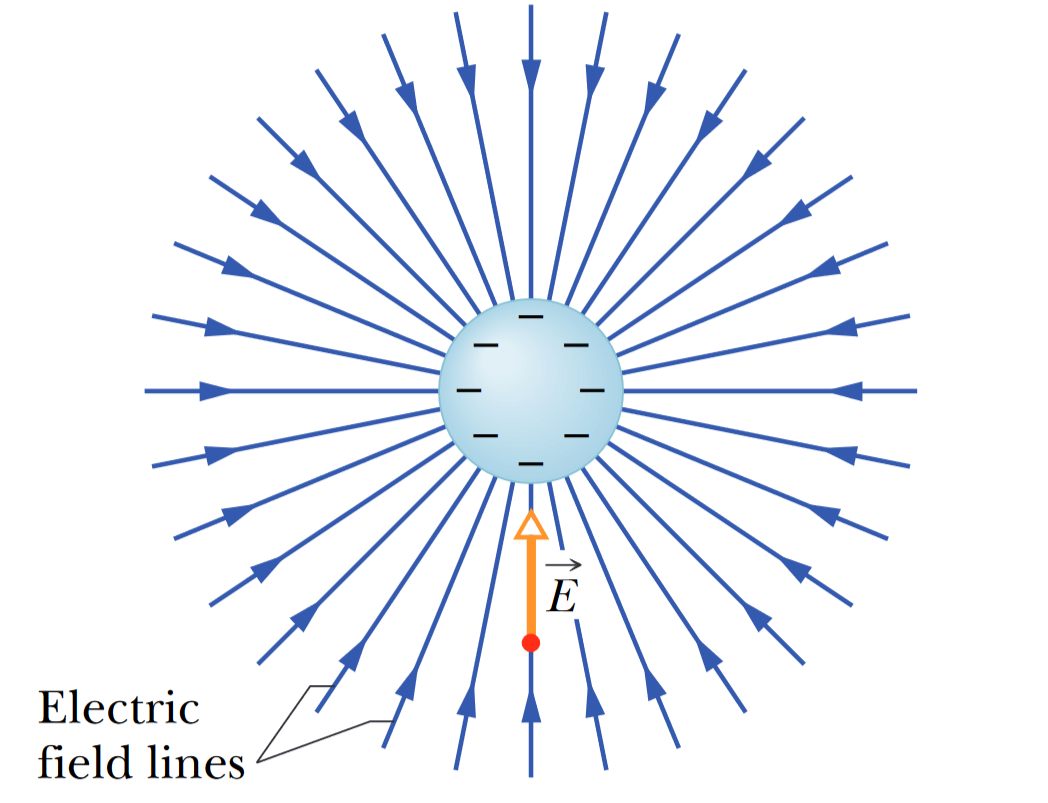
\includegraphics[width=8cm]{Physics2_PNGs/elec-field-lines.png}
			\caption{Electric Field Lines}
			\label{fig:electric-field-lines}
		\end{figure}
		
		
		\subsection*{2.1 Electric Fiels due to a Point Charge}
		To find an electric charge due to a point $q$ at any point to a distance $r$, we put a positive charge $q_0$. The \textbf{electrostatic force} acting on $q_0$ is:
		\begin{equation*}
			\vec{F} = \frac{1}{4\pi\varepsilon_0} \frac{q q_0}{r^2} \hat{r} 
		\end{equation*}
		The direction of $\vec{F}$ points directly away from the point charge is $q$ is positive, towards the point charge if $q$ is negative.
		The \textbf{electric field vector} is:
		\begin{equation*}
			\vec{E} = \frac{\vec{F}}{q_0} = \frac{1}{4\pi\varepsilon_0} \frac{q}{r^2} \tag{Point Charge, 2-2}
		\end{equation*}	
		$\vec{E}$ and $\vec{F}$ have same direction.
		
		We can quickly find the resultant electric field due to more than one point
		charge by placing a positive charge $q_0$ near $n$ point charges $q_1, q_2, . . . , q_n$, then,
		from Eq. 1-5, the net force from the n point charges acting on the test charge is:
		\begin{equation*}
			\vec{F_{0}} = \vec{F_{01}} + \vec{F_{02}} + \vec{F_{03}} + ... + \vec{F_{0n}}.
		\end{equation*}
		Therefore the net electric field at the position of the charge is:
		\begin{equation*}
			\vec{E} = \frac{\vec{F_0}}{q_0} = \frac{\vec{F_{01}}}{q_0} + \frac{\vec{F_{02}}}{q_0} + ... + \frac{\vec{F_{0n}}}{q_0} = \sum_{i=1}^{n} \frac{\vec{F_{0i}}}{q_0} = \sum_{i=1}^{n} \vec{E_i} \tag{2-3}
		\end{equation*}
	
		
		\subsection*{2.2 Electric Field due to an Electric Dipole}
		
		\begin{wrapfigure}{r}{0.25\textwidth}
			\centering
			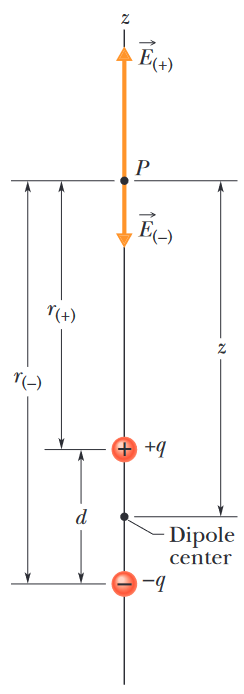
\includegraphics[width=3.5cm]{Physics2_PNGs/elec-dipole.png}
			\caption{An Electric Dipole}
			\label{fig:electric-dipole}
		\end{wrapfigure}
	
		An \textbf{Electric Dipole} consists of two charges of magnitude $q$, but opposite signs, separated by a distance $d$. The point of interest $P$ is located along the the \textbf{Dipole Axis} at a distance \textit{z} from the dipole's midpoint. 
		
		Due to the simmetry of this setup, the electric field components from the two charges ($E_{+}$ and $E_{-}$) must lie along the dipole axis which we have taken to be \textit{z} axis. Applying the \textbf{superposition principle} for electric fields, we find that the magnitude \textbf{E} at a point $P$ is: 
		\begin{equation*}
			\textbf{E} = E_{+} + E_{-}
		\end{equation*}
		\begin{equation*}
			= \frac{1}{4\pi \varepsilon_0} \frac{q}{r^2_{(+)}} - \frac{1}{4\pi \varepsilon_0} \frac{q}{r^2_{(-)}}
		\end{equation*}
		\begin{equation*}
			= \frac{q}{4\pi \varepsilon_0(\textit{z}-\frac{1}{2}d)^2} - \frac{q}{4\pi \varepsilon_0(\textit{z}+\frac{1}{2}d)^2}.
		\end{equation*}
		With a little algebra:
		\begin{equation*}
			\textbf{E} = \frac{q}{4\pi\epsilon_0\textit{z}^2}\biggl(\frac{1}{(1-\frac{d}{2\textit{z}})^2 } - 
			\frac{1}{(1+\frac{d}{2\textit{z}})^2 }\biggl).
		\end{equation*}
		\begin{equation*}
			\textbf{E} = 
			\frac{q}{4\pi \varepsilon_0\textit{z}^2} 
			\frac{2d/ \textit{z}}{\small(1-(\frac{d}{2\textit{z}})^2)^2}
			= \frac{q}{2\pi \varepsilon_0\textit{z}^3} 
			  \frac{d}{ (1 - (\frac{d}{2\textit{z}})^2)^2 }
			  \tag{2-4}
		\end{equation*}
	
		We are usually interested in the electrical effect of the dipole only at distances larger than the dipole, such distances as $\textit{z} \gg d$.
		At such distances, we have $d/2\textit{z} \ll 1$ in Eq. 2-4. Given this approximation, we can rewrite 2-4 as:
		\begin{equation*}
			\textbf{E} = \frac{1}{2\pi\varepsilon_0} \frac{qd}{\textit{z}^3}
			\tag{2-5}
		\end{equation*}
		
		The product $qd$ is the magnitude $\textbf{p}$ of a vector called  \textbf{Electric Dipole Moment} ($\vec{p} = q\vec{d}$). Thus we can rewrite 2-5 as:
		\begin{equation*}
			\textbf{E} = \frac{1}{2\pi\varepsilon_0} \frac{p}{\textit{z}^3}
			\tag{Electric Dipole, 2-6}
		\end{equation*}
		The direction of $\vec{p}$ is taken to be from the negative to the positive side of the dipole.
		
		
		\subsection*{2.3 Electric Field due to a Line of Charge}
		
		\begin{wraptable}{r}{0pt} 
			
			$ \begin{array}{crrr}
				 Name & Symbol & \text{SI Unit} \\
				\toprule
				Charge & q & C \\
				\text{Linear Charge Density} & \lambda & C/m \\
				\text{Surface Charge Density} & \sigma & C/m^2 \\
				\text{Volume Charge Density} & \rho & C/m^3 \\
				\bottomrule
			\end{array} $
			\caption{Some Measures of Electric Charge}
		\end{wraptable}
		
		We now consider \textbf{continuous} charge distributions. Given a ring of radius $R$ of uniform positive linear charge density $\lambda$ around its circumference, a differential element of charge occupies a length $ds$. This element sets up an electrical field $d\vec{E}$ at a point $P$. The component of $d\vec{E}$ along the central axis can be intercepted by $dE\cos\theta$.
		Therefore every element $ds$ has a charge of magnitude 
		\begin{equation*}
			dq = \lambda ds \tag{2-6}
		\end{equation*}
		This differential charge sets up a differential electric field $\vec{E}$ at a point $P$, which is at a distance $r$ from the point. Using Eq. 2-6 we can rewrite Eq. 2-2:
		\begin{equation*}
			dE = \frac{1}{4\pi\varepsilon_0} \frac{dq}{r^2} 
			   = \frac{1}{4\pi\varepsilon_0} \frac{\lambda ds}{r^2}
			   \tag{22-7}
		\end{equation*}
		
		\begin{wrapfigure}{r}{0.25\textwidth}
			\centering
			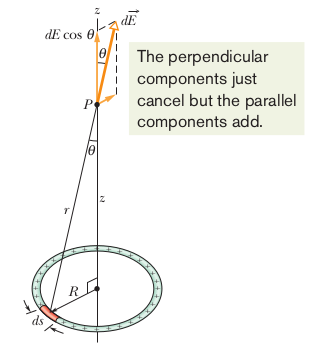
\includegraphics[width=6.07cm]{Physics2_PNGs/elec-line-charge.png}
			\caption{A Ring of Uniform Positive Charge}
			\label{fig:electric-line-of-charge}
		\end{wrapfigure}
		From Figure 3 we can rewrite Eq. 2-7: 
		\begin{equation*}
			dE = \frac{1}{4\pi\varepsilon_0} \frac{\lambda ds}{(\textit{z}^2 + R^2)}
				\tag{2-8}
		\end{equation*}
		Every $d\vec{E}$ has a component perpendicular to the central axis $\textit{z}$ ($d\vec{E}\cos\theta$) with equal magnitude but different direction. \\
		Therefore: 
		
		\begin{equation*}
			\begin{cases}
				\cos\theta = \scalebox{1.6}{$ \frac{\textit{z}}{r} $} = 
				\scalebox{1.4}{$ 
					\frac{\textit{z}}{(\textit{z}^2 + R^2)^{1/2}} $} \\ \\
				dE = \scalebox{1.3}{$\frac{1}{4\pi\varepsilon_0} \frac{\lambda ds}{(\textit{z}^2 + R^2)} $}
			\end{cases}\,.
		\end{equation*}
	
		Multiplying the first expression for the second gives us:
		\begin{equation*}
			d\vec{E}\cos\theta = \frac{\textit{z}\lambda}{4\pi\varepsilon_0(\textit{z}^2+R^2)^{3/2}}ds
			\tag{2-9}
		\end{equation*}
		
		To add the parallel components ($dE\cos\theta$) produced by all elements we integrate Eq. 2-9 around the circumference of the ring, from $s = 0$ to $s = 2\pi R$:
		\begin{equation*}
			E = \int dE\cos\theta = \frac{\textit{z}\lambda}{4\pi\varepsilon_0(\textit{z}^2+R^2)^{3/2}} \cdot
			\int_{0}^{2\pi R}ds = 
 			\frac{\textit{z}\lambda (2\pi R)}{4\pi\varepsilon_0(\textit{z}^2 + R^2)^{3/2}} 
			\tag{2-10}
		\end{equation*} 
		Since $\lambda$ is the charge per length of a ring, the term $\lambda2\pi R$ is just $q$ [$q = \lambda(2\pi R)$]:
		\begin{equation*}
			\scalebox{1.1}{$E$} = 
				\frac{\scalebox{1.2}{$q\textit{z}$}}
				     {\scalebox{1.3}{$4\pi\varepsilon_0(\textit{z}^2 + R^2)^{3/2}$}}
			\tag{Charged Ring, 2-11}
		\end{equation*}
		This equation yields the same results even if $q$ is negative. \\
		If we assume that $\textit{z} \gg R$, $\textit{z}^2 + R^2$ can be approximated as $\textit{z}^2$ and 2-11 becomes:
		\begin{equation*}
			E = \frac{q\textit{z}}{4\pi\varepsilon_0 \textit{z}^2} 
			\tag{Charged Ring at Large Distances, 2-12}
		\end{equation*}
		
		
		\subsection*{2.3.1 A Field Guide for Lines of Charge}
		Finding the electric field $\vec{E}$ produced at a point $P$ by a line of uniform charge, either circular or straight. The strategy is to pick on an element $dq$ of charge, find $d\vec{E}$ due to that element and integrate $d\vec{E}$ over the entire line of charge.
		\begin{itemize}
			\item[\textbf{Step 1.}] If the line of charge is circular, let $ds$ be the arc length of an element of the distribution. If the line is straight, sum on $x$ axis along it and let $dx$ be the length of an element.
			
			\item[\textbf{Step 2.}] Relate $dq$ of the element to the length of the element with either $dq = \lambda ds$ or $dq = \lambda dx$. Consider $dq$ and $\lambda$ positive even if the charge is actually negative.
			
			\item[\textbf{Step 3.}] Express the field $d\vec{E}$ produced at $P$ by $dq$ with
			$\vec{E} = \frac{\vec{F}}{q_0} = \frac{q}{4\pi\varepsilon_0r^2}$, replacing $q$ with either $q = \lambda ds$ or $q = \lambda dx$. If the charge on the line is positive then at $P$ draw a vector $d\vec{E}$ that points directly away from $dq$, opposite if the charge is negative.
			
			\item[\textbf{Step 4.}] Always look for any simmetry in the situation. If $P$ is on an axis of simmetry of the charge distribution, resolve the field $d\vec{E}$ produced by $dq$ into components that are perpendicular and parallel to the axis of simmetry. Repeat with the simmetric element $dq'$ and draw the vector $d\vec{E}'$ at $P$. One of the components produced by $dq$ is a cancelling component, cancelled by the corrisponding component produced by $dq'$, we have a similar concept in adding components. Integration is a way to add them up.
			
			\item[\textbf{Step 5.}] There are four general types of uniform charge distribution:
				\begin{itemize} 
					\item[Ring:] With point $P$ on the central axis of simmetry. In the expression for $d\vec{E}$ replace $r^2 = \textit{z}^2 + R^2$. Express the adding components of $d\vec{E}$ in terms of $\theta$. That introduces $\cos\theta$, but $\theta$ is identical to all the elements, therefore is not a variable. Replace $\cos\theta = \frac{\textit{z}}{r} = \frac{\textit{z}}{(\textit{z}^2 + R^2)^{1/2}}$ and integrate over $s$ around the circumference.
					
					\item[Circular Arc:] Point $P$ at the center of the curvature. Express the adding component of $d\vec{E}$ in terms of $\theta$. That introduces either $\sin\theta$ or $\cos\theta$. Reduce the two resulting variables $s$ and $\theta$ by replacing $ds = rd\theta$ from one end of the arc to the other.
					
					\item[Straight Line:] with point $P$ on an extension of the line (as in Fig. 4a). In the expression for $dE$, replace $r$ with $x$. Integrate over $x$ from end to end.	
					
					\item[Straight Line:] with point P at perpendicular distance $y$ from the line of charge  (Fig. 4b). In the expression for $dE$ replace $r$ with an expression involving $x$ and $y$. If $P$ is on the perpendicular bisector of the line of charge, find an expression for the adding component of $d\vec{E}$. That will introduce either $\sin\theta$ or $\cos\theta$. Reduce the resulting two variables $x$ and $\theta$ to one, $x$, by replacing the trigonometric function with an expression involving $x$ and $y$. Integrate over $x$ from end to end of the line of charge. If $P$ (Fig. 4c) is not on the line of simmetry, set up an integral to sum the components $dE_x$ and integrate over $x$ to find $E_x$. Also set up an integral to sum the components $dE_y$, integrate over $x$ again to find $E_y$. Now use $E_x$ and $E_y$ to find magnitude and direction of $\vec{E}$.
					
				\end{itemize}
			
			\item[\textbf{Step 6.}] One arrangement of the integration limits gives a positive result. The reverse gives the same result with a minus sign. Discard the minus sign. If the result is to be stated in terms of the total charge $Q$ of the distribution, replace $\lambda = Q / L$ in which $L$ is the length of the distribution.
			
		\end{itemize}
	
		\begin{figure}
			\centering
			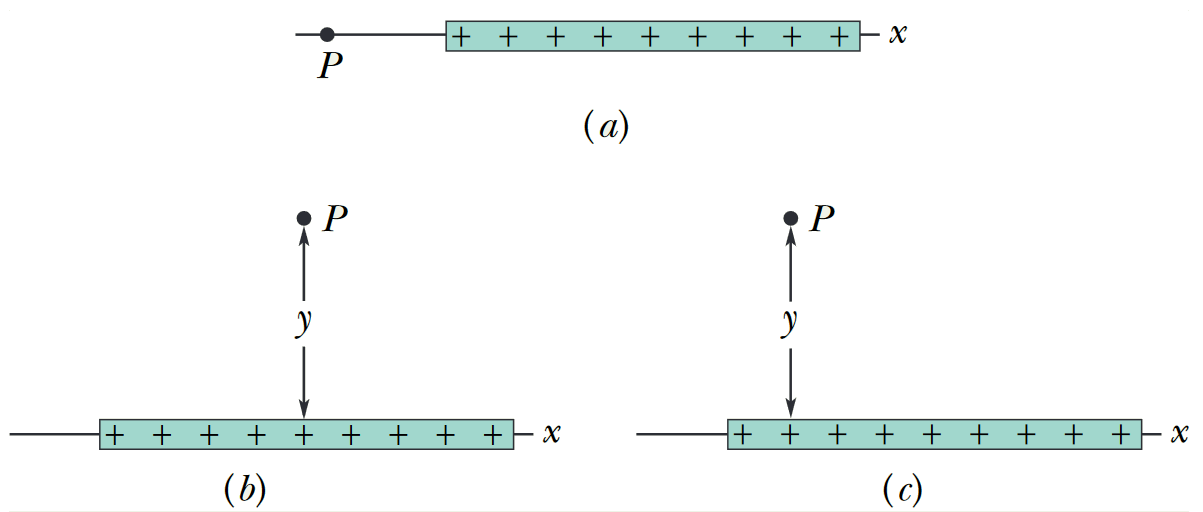
\includegraphics[width=10cm]{Physics2_PNGs/electric-line-charge.png}
			\caption*{Figure 4}
			\label{fig:line-of-charge}
		\end{figure}
	
	
		\subsection*{2.4 Point Charge in an Electric Field}
		
		\begin{wrapfigure}{r}{0.25\textwidth}
			\centering
			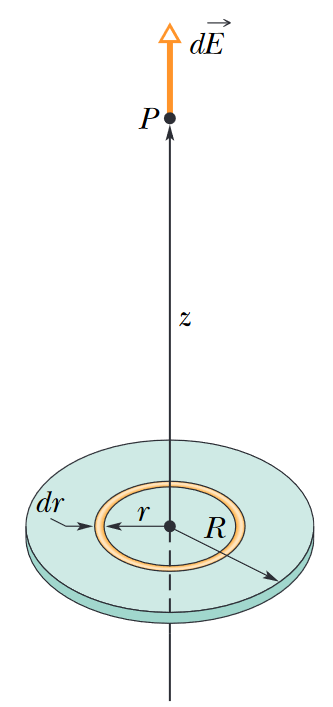
\includegraphics[width=3cm]{Physics2_PNGs/elec-charged-disk.png}
			\caption*{Figure 5: A disk of uniform positive charge}
			\label{fig:charged-disk}
		\end{wrapfigure}
	
		Figure 4 shows a circular plastic disk of $radius$ $R$ that has a positive surface charge of uniform density $\sigma$ on its upper surface. We need to find the electric field at point $P$, with distance $z$ from the disk along its central axis.
		We divide the disk into concentric flat rings and then calculate the electric field at point $P$ by adding up (integrating) the contribution of all rings. Fig. 4 shows one such ring, with radius $r$ and radial width $dr$. The charge on the ring is:
		
		\begin{equation*}
			dq = \sigma dA = \sigma (2\pi rdr)
			\tag{2-13}
		\end{equation*} 
		
		where $dA$ is the differential area of the ring. \\
		Substituting $dq$ from Eq. 2-13 for $q$ in Eq. 2-11:
		
		\begin{equation*}
			dE = \frac{z\sigma 2 \pi rdr}{4\pi\varepsilon_0(z^2 + r^2)^{3/2}}
		\end{equation*}
		which we can rewrite as
		\begin{equation*}
			dE = \frac{\sigma z}{4\varepsilon_0} \frac{2rdr}{(z^2 + r^2)^{3/2}}
			\tag{2-14}
		\end{equation*}
	
		We can now find $E$ by integrating 2-14 over the surface of the disk, with respect to the variable $r$ from $r = 0$ to $r = R$. We get
		\begin{equation*}
			E = \int dE = \frac{\sigma z}{4\varepsilon_0} \int_{0}^{R} (z^2 + r^2)^{-3/2}(2r)dr
			\tag{2-15}
		\end{equation*}
	
		This is easily solvable by casting the integral in the form $\int X^mdX$, by setting \\ $X = (z^2 + r^2),\quad dX = (2rdr)$  and  $ m = -\frac{3}{2}$, we have
		\begin{equation*}
			\int X^m dX = \frac{X^{m+1}}{m+1}
		\end{equation*}
	
		The solved integral becomes
		\begin{equation*}
			E = \frac{\sigma z}{4\varepsilon_0} \biggl[\frac{(z^2 + r^2)^{-1/2}}{-\frac{1}{2}} \biggl]_{0}^{R}
			\tag{2-16}
		\end{equation*}
	
		Taking the limits and rearranging we obtain:
		\begin{equation*}
			\textit{\textbf{E}} = \frac{\sigma}{2\varepsilon_0} \biggl(1 - \frac{z}{\sqrt{z^2 + R^2}} \biggl)
			\tag{Charged Disk, 2-17}
		\end{equation*}
		
		If we let $R \rightarrow \infty$ while keeping $z$ finite, the equation reduces to
		\begin{equation*}
			E = \frac{\sigma}{2\varepsilon_0}
			\tag{2-18}
		\end{equation*}
		This is the electric field produced by an infinite sheet of uniform charge. We get the same result by letting $z \rightarrow 0$ while keeping $R$ finite.
		
		
		
		\subsection*{2.5 Point Charge in an Electric Field}
		
		\begin{equation*}
			\vec{F} = q\vec{E}
			\tag{2-19}
		\end{equation*}
		
		The electrostatic force $\vec{F}$ acting on a charged particle located in an external electric field $\vec{E}$ has the direction of $\vec{E}$ if the charge $q$ of the particle is positive and has the opposite direction if $q$ is negative.
		
		
		\subsection*{2.6 A Dipole in an Electric Field}
		
		We have defined Dipole Moment ($\vec{p} =q\vec{d}$) as a vector that point from the negative to the positive end of the dipole. 
		A dipole in an Electric Field $\vec{E}$ consists of a rigid structure with two center of opposite charge and magnitude $q$. The dipole moment $\vec{p}$ makes an angle $\theta$ with $\vec{E}$. Electrostatic forces act on the charged ends of the dipole. Since $\vec{E}$ is uniform, those forces act in opposite directions with magnitude $F = qE$. Thus, since the field is uniform, the \textit{net force} on the dipole is $= 0$. However the forces on the charged ends produce a \textbf{net torque} $\vec{\tau}$ on the dipole in his center of mass, which lies in the line connecting the charged ends at some distance $x$ from one end and thus a distance $d - x$ from the other end. \\
		Given $\tau = rF\sin\phi$ we can write the magnitude of the net torque as:
		\begin{equation*}
			\tau = Fx\sin\theta + F(d-x)\sin\theta = Fd\sin\theta
			\tag{2-20}
		\end{equation*}
		or, by substituting $F = qE$ and $d = p / q$ we can find the magnitude of $\vec{\tau}$:
		\begin{equation*}
			\tau = pE\sin\theta
			\tag{2-21}
		\end{equation*}
		In a generalized vector form:
		\begin{equation*}
			\vec{\tau} = \vec{p} \times \vec{E}
			\tag{Torque on a Dipole, 2-22}
		\end{equation*}
	
		\begin{figure}
			\centering
			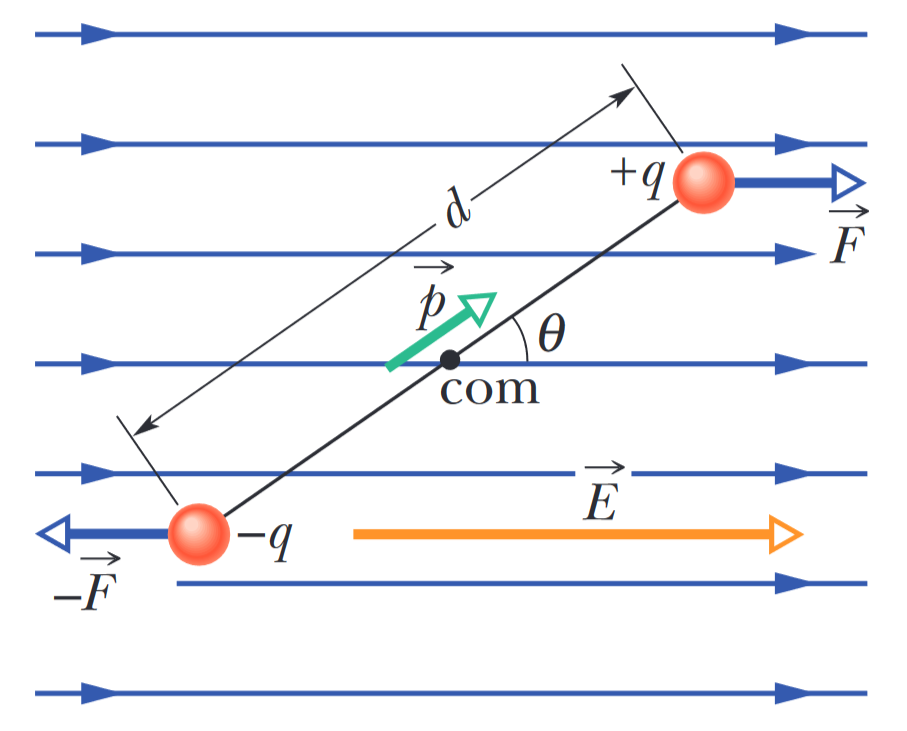
\includegraphics[width=5cm]{Physics2_PNGs/potential-dipole.png}
			\caption*{Figure 6: Dipole in an uniform external electric field $\vec{E}$}
			\label{fig:potential-dipole}
		\end{figure}
		
		
		\subsection*{2.7 Potential Energy of an Electric Dipole}
		
		We can associate potential energy with the orientaton of an electric dipole in an electric field. \\
		The dipole has less potential energy when it's in equilibrium orientation. Therefore when $\vec{\tau} = \vec{p} \times \vec{E} = 0$. The dipole is like a pendulum, which has the least gravitational potential energy in its equilibrium orientation. In any situation involvint potential energy we are free to define the 0 potential energy configuration. Given $\Delta U = -W$ and $W = \int \tau d\theta$ we find the potential energy at any angle $\theta$ to be:
		\begin{equation*}
			U = -W = -\int_{90^\circ}^{\theta} \tau d\theta = \int_{90^\circ}^{\theta} pE\sin\theta d\theta
			\tag{2-23}
		\end{equation*}
		Evaluating the integral leads to:
		\begin{equation*}
			U = -pE\cos\theta
			\tag{2-24}
		\end{equation*}
		We can generalize this equation in vectorial form as
		\begin{equation*}
			U = -\vec{p} \cdot \vec{E}
			\tag{Potential Energy of a Dipole, 2-25}
		\end{equation*}
		
		
		\newpage
		\section*{3. Gauss' Law}
		
		
		Gauss’ law relates the electric fields at points on a (closed) Gaussian surface to the net charge enclosed by that surface.
		
		
		\subsection*{3.1 Flux}
		
		Let's suppose a wide airstream of uniform velocity $\vec{v}$ at a small square loop of area $A$. Let \textbf{$\Phi$} represent the \textit{volume flow rate} at which the air flows thorugh the loop and let $\theta$ be the angle between the velocity $\vec{v}$ and the area vector $\vec{A}$ (a vector whose magnitude is equal to $A$ and whose direction is normal to the plane of the area $A$). We can now say that:
		\begin{equation*}
			\textbf{$\Phi$} = (v\cos\theta)A = \vec{v} \cdot \vec{A}
			\tag{3-1}
		\end{equation*}
		
		\begin{figure}[!htb]  % force figure under subsection
			\centering
			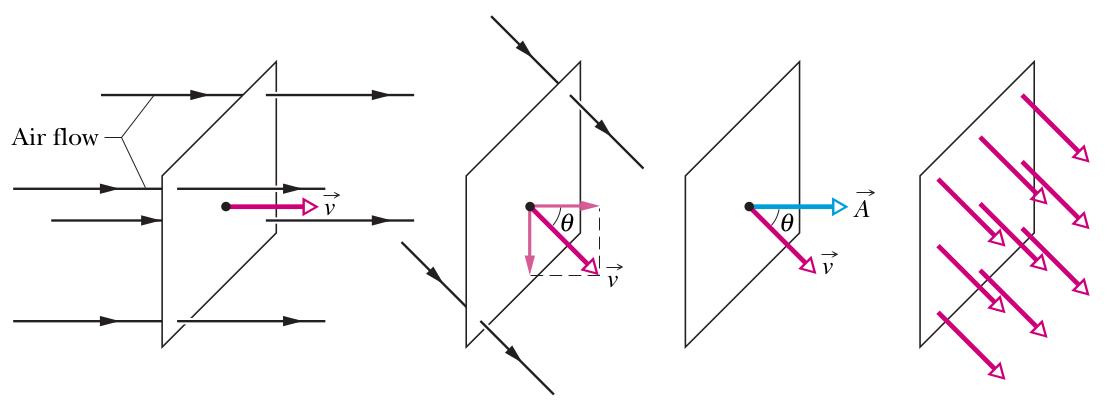
\includegraphics[width=10cm,height=3.5cm]{Physics2_PNGs/elec-veloc-flux.png}
			\caption*{Figure 7: An airstream $\vec{v}$ going through a square of area $A$}
			\label{fig:flux-over-square}
		\end{figure}
	
	
		\subsection*{3.2 Flux of an Electric Field}
		
		\begin{wrapfigure}{r}{0.15\textwidth}
			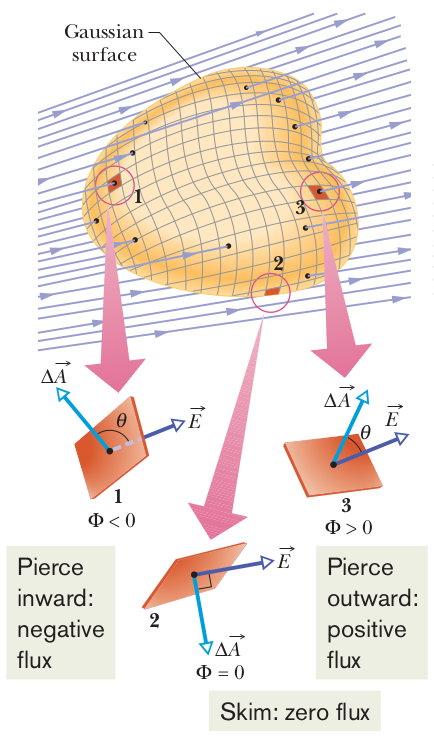
\includegraphics[width=4.5cm,height=7cm]{Physics2_PNGs/gaussian-elec-field.png}
			
			\label{fig:gaussian-elec-field}
		\end{wrapfigure}
		
		To define the flux of an electric field, we can take an arbitrary (asymmetric) Gaussian Surface immersed in a nonuniform electric field. Let us divide the surface into small squares of area $\Delta A$, small enough to neglect the curvature of the surface. We represent each of such element with an area vector $\Delta\vec{A}$.
		Given the small dimension of each square, we can treat the electric field $\vec{E}$ as constant over any given square. The vector $\Delta\vec{A}$ and $\vec{E}$ for each square make some angle $\theta$ with each other. A first definition for the flux of the electric field for a Gaussian Surface can be:
		\begin{equation*}
			\Phi = \sum \vec{E} \cdot \Delta\vec{A}
			\tag{3-2}
		\end{equation*}
		If we allow the area of each square to become smaller and smaller, we can approach a differential limit $dA$. The area vectors will therefore approach a differential limit $d\vec{A}$. \\ \\The sum 3-2 becomes a closed surface integral:
		\begin{equation*}
			\scalebox{1.3}{$ \mathbf{\Phi} = \bigointsss \vec{E} \cdot d\vec{A}$ }
			\tag{Electric Flux through a Gaussian Surface, 3-3}
		\end{equation*}
		The Flux of an Electric Field is a \textit{scalar}, and its \textbf{SI} unit is the \textit{newton-square-meter per coulomb} [$N \cdot m^2/C$] 
		
		\newpage
		\subsection*{3.2.1 Flux through a Closed Cylinder, Uniform Field}
		
		Given a \textbf{Cylinder}-shaped Gaussian Surface, with radius $R$ immersed in an \textbf{uniform} electric field $\vec{E}$, with the cylider axis parallel to the field. What is the flux $\mathbf{\Phi}$ of the electric field through this closed surface? \\
		We can find the flux $\mathbf{\Phi}$ by \textbf{integrating} the scalar product $\vec{E} \cdot d\vec{A}$ over the surface.
		We can do the integration by writing the flux as the sum of three terms: left cylinder cap $a$, the cylindrical surface $b$, right cylinder cap $c$. Thus:
		\begin{gather*}	% equation with newline
			\Phi = \bigointssss \vec{E} \cdot d\vec{A} 
			= \bigintssss_{a} \vec{E} \cdot d\vec{A}
			+ \bigintssss_{b} \vec{E} \cdot d\vec{A}
			+ \bigintssss_{c} \vec{E} \cdot d\vec{A} 	\tag{3-4} \\
				\bigintssss_{a} \vec{E} \cdot d\vec{A} 
					= \bigintssss_{a} E(\cos180^\circ) dA = E \cdot A = -\pi R^2 E	\\
				\bigintssss_{b} \vec{E} \cdot d\vec{A}  
					= \bigintssss_{b} E(\cos90^\circ) dA = 0	\\
				\bigintssss_{c} \vec{E} \cdot d\vec{A} 
					= \bigintssss_{a} E(\cos0^\circ) dA = E \cdot A = \pi R^2 E	\\
			\text	{Substituting into 3-4 yields:}  \\
			\Phi = -\pi R^2 E + 0 + \pi R^2 E = 0 \tag{Answer}
		\end{gather*}
		
		\begin{figure}[!htb]  % force figure under subsection
			\centering
			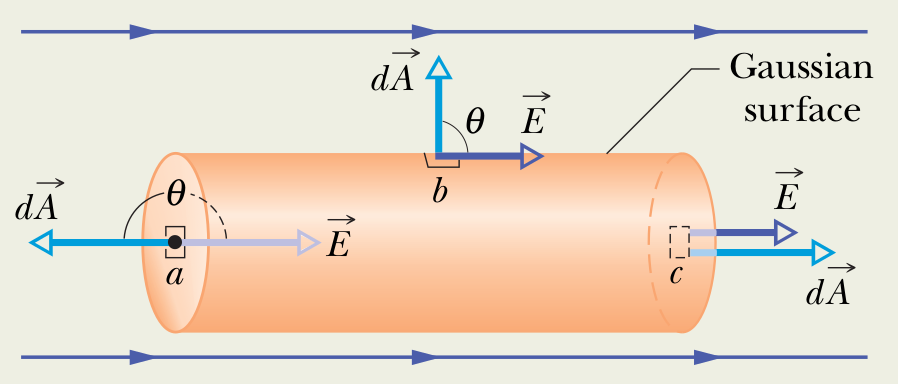
\includegraphics[width=8cm]{Physics2_PNGs/closed-cylinder.png}
			\caption*{}
			\label{fig:closed-cylinder}
		\end{figure}
		The net flux is zero because the field lines that represent the electric field all pass entirely through the Gaussian surface, from the left to the right.
		
		
		\subsection*{3.3 Gauss' Law}
		
		Gauss' Law relates the net flux $\Phi$ of an electric field through a closed surface (a Gaussian Surface) to the net charge $q_{enc}$ that is \textit{enclosed} by that surface. It tells us that:
		\begin{equation*}
			\varepsilon_0 \Phi = q_{\text{int}}
			\tag{Gauss' Law, 3-5}
		\end{equation*}
		By substituting 3-5 into the definition of Flux, we can also write Gauss' Law as:
		\begin{equation*}
			\varepsilon_0 \bigointssss \vec{E} \cdot d\vec{A} = q_{\text{int}}
			\tag{Gauss' Law, 3-6} 
		\end{equation*}
		These equations holds when the net charge is located in the void or in the air. The net charge $q_{enc}$ is the algebraic sum of all \textit{enclosed} positive and negative charges. \\ 
		If $q_{\text{int}} > 0$ the net flux is \textit{outward}; \\
		if $q_{\text{int}} < 0$ the net flus is \textit{inward}. \\
		Charges \text{outside} the surface are not included in the term $q_{\text{int}}$ in Gauss' Law. The exact form and location of the charges of the Gaussian Surface are also irrelevant. The only thing that matters on the right side of the equations are the magnitude and sign of the net enclosed charge. \\
		However the quantity $\vec{E}$ on the left side of Eq. 3-6 is the electric field resulting from all charges, both those inside and those outside the Gaussian Surface, this is due to the fact that the electric field due to a charge outside the Gaussian surface contributes zero net flux through the surface, because as many field lines due to that charge enter the surface as leave it. \\
		
		\begin{wrapfigure}{r}{0.17\textwidth}
			\centering
			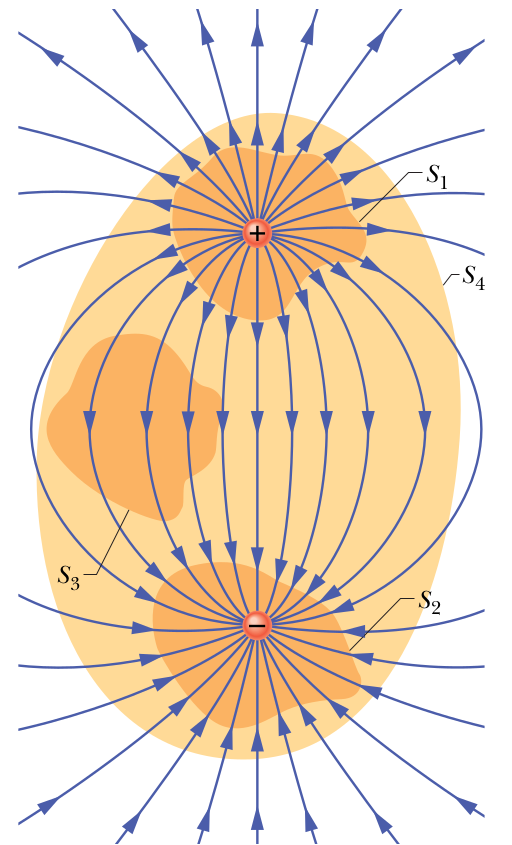
\includegraphics[width=4cm]{Physics2_PNGs/gaussian-surf-lines.png}
			\caption*{Figure 8}
			\label{gaussian-surf-lines}
		\end{wrapfigure}
		
		In Fig. 8 we have an example of two charges of \textbf{equal magnitude}, but \textbf{opposite sign}. Four Gaussian Surfaces are shown in cross section:
		\begin{itemize}
			\item[Surface $S_1$]: $\vec{E}$ is outward for all points, thus flux $\Phi > 0$ and $q_{\text{int}} > 0$.
			\item[Surface $S_2$]: $\vec{E}$ is inward for all points, thus flux $\Phi < 0$ and $q_{\text{int}} < 0$.
			\item[Surface $S_3$]: This surface encloses no charge, thus $q_{\text{int}} = 0$, by Gauss' Law also requires that net flux $\Phi = 0$.
			\item[Surface $S_4$]: This surface encloses no \textit{net} charge, because the enclosed positive and negative charges have equal magnitudes \\ 
			($q_{\text{int}} = q_1 - q_2 = 0$). Gauss' Law requires that net flux $\Phi = 0$.
		\end{itemize}
		\ \\ \\ 		
		
		\subsection*{3.4 Gauss' Law and Coulomb's Law}
		
		Since Coulomb's Law and Gauss' Law are different ways of describing the relationship between \textbf{electric charge} and \textbf{electric field} in static situations, we should be able to derive each from the other. \\
		Taken a positive point charge $q$ around which we drawn a concentric Gaussian surface of radius $r$. We can divide the surface into differential areas $dA$. By definition the area vector $d\vec{A}$ is perpendicular and pointed outwards at any point of the surface. From the simmetry of the situation, we know that the field $\vec{E}$ is also perpendicular to the surface and directed outward. Thus, since the angle $\theta$ between $\vec{E}$ and $d\vec{A}$ is zero, we can rewrite Eq. 3-6 for Gauss' Law as: 
		
		\begin{equation*}
			\varepsilon_0 \oint \vec{E} \cdot d\vec{A} =
			\varepsilon_0 \oint EdA = q_{\text{int}}
			\tag{3-7}
		\end{equation*}

		Here, $q_{\text{int}} = q$. Although $E$ varies radially with distance from $q$, it has same value everywhere on the spherical surface. We can draw the conclusion that E is constant, therefore:
		
		\begin{equation*}
			\varepsilon_0 E \oint dA = q.
		\end{equation*}
	
		The integral now is just the sum of all the points on the surface of the sphere, we can then rewrite the differential $dA$ over the surface of the sphere as ($4\pi r^2)$:
		
		\begin{equation*}
			\varepsilon_0 E (4\pi r^2) = q
		\end{equation*}
	
		or, rearranging:
		
		\begin{equation*}
			E = \frac{1}{4\pi\varepsilon_0} \frac{q}{r^2}
			\tag{3-8}
		\end{equation*}
		We can observe that the resulting equation is coherent with Coulomb's Law.


		
		\subsection*{3.5 A Charged Isolated Conductor}

		If an excess charge is placed on an isolated conductor, that amount of charge will move entirely to the surface of the conductor, thus none of the excess charge will be found within the body of the conductor ( Given by the fact that charges with same sign repel one another ).\\
		We take a Gaussian Surface just under the Conductor's Surface \\
		\begin{equation*}
			E = 0 \rightarrow \Phi = 0 \rightarrow q_{int} = 0 
		\end{equation*}
		The excess charge over an Isolated Conductor lays completely over the external surface.  \\\\
		The same principle applies to an Isolated Conductor with a cavity, its surface has no \text{excess} charge.
		
		
		\subsection*{3.6 External Electric Field}
		
		
		\begin{wrapfigure}{r}{0.17\textwidth}
			\centering
			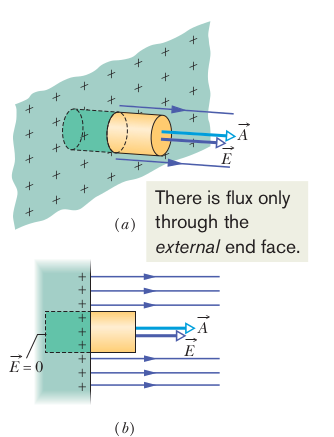
\includegraphics[width=5cm]{Physics2_PNGs/external-elec-field.png}
			\caption*{}
			\label{fig:external-elec-field.png}
		\end{wrapfigure}
		
		Overall, the charge does not distribute evenly over the Surface of a Conductor. 
	
		Eventhough there's a direct relationship between the field $\vec{E}$ and the (surface) Charge Density $\sigma$ $[ C/m^2 ]$.\\
		We take a small cylinder that encapsulates an element of the Surface. The field $\vec{E}$ is \textbf{perpendicular} to the surface (the charge would move otherwise). Therefore the charge $q_{\text{int}}$ enclosed by the Gaussian surface lies on the conductor's surface in an area $A$. Knowing that $\sigma$ is the charge per unit area, then $q_{\text{int}}$ is equal to $\sigma A$. Substituting $\sigma A$ for $q_{int}$ and $EA$ for $\Phi$, Gauss' law becomes:
		\begin{equation*}
			\varepsilon_0 EA = \sigma A 
			\tag{3-9}
		\end{equation*}
		from which we find:
		\begin{equation*}
			E = \frac{\sigma}{\varepsilon_0}
			\tag{Conducting Surface, 3-10}
		\end{equation*}
	
		\newpage
	
	
	
		\subsection*{3.7 Gauss' Law: Cylindrical Symmetry}
		
		Infinitely long cylindrical plastic rod with uniform positive linear charge density $\lambda$ $[ C/m ]$. Let's find an expression for the magnitude of the Electric field $\vec{E}$ at a distance $r$ from the axis of the rod. The Gaussian Surface we choose should match the simmetry of the problem (which is cylindrical).
		
		We choose a circular cylinder of radius $r$ and length $h$, coaxial with the rod. Any rotation of the rod (about its longitudinal axis) wouldn't make any change in the electric field. Therefore at every point on the cylindrical part of the Gaussian surface $\vec{E}$ must have the same magnitude $E$ and must directed radially outside (for a positively charged rod). \\
		
		Since $2\pi r$ is the cylinder circumference and $h$ is its height, the area A of the cylindrical surface is $2\pi rh$. The flux $\vec{E}$ through the surface is then
		\begin{equation*}
			\Phi = EA\cos\theta = E(2\pi rh)\cos0 = E(2\pi rh)
		\end{equation*}
		There is no flux through the end caps of the surface since $\vec{E}$ is radially directed, thus parallel to the end caps at every point.
		
		The charge enclosed by the surface is $\lambda h$, therefore
		\begin{equation*}
			\varepsilon_0 \Phi = q_{\text{int}}
		\end{equation*}
		reduces to
		\begin{equation*}
			\varepsilon_0 E(2\pi rh) = \lambda h
		\end{equation*}
	
		We can then describe the field around an infinitely long, straight rod of charge as
		\begin{equation*}
			E = \frac{\lambda}{2\pi\epsilon_0 r}
			\tag{line of charge, 3-11}
		\end{equation*}
	
		
	
	
		\subsection*{3.8 Gauss' Law: Planar Symmetry}
		
		\begin{wrapfigure}{r}{0.17\textwidth}
			\centering
			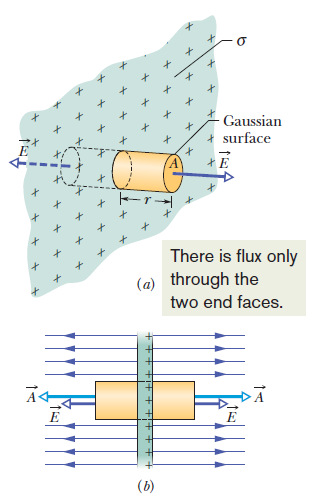
\includegraphics[width=4cm]{Physics2_PNGs/planar-gauss-surf.png}
			\caption*{}
			\label{fig:planar-gauss-surf.png}
		\end{wrapfigure}
		
		
		Thin, infinite, non-conducing sheet with an uniform (positive) surface charge density $\sigma$ $[ C/m^2 ]$. A useful Gaussian surface is a closed cylinder with end caps of area $A$, arranged to pierce the sheet perpendicularly as shown. From symmetry, $\vec{E}$ must be perpendicular to the sheet and hence to the end caps. Furthermore, since the charge is positive, $\vec{E}$ is directed \textit{away} from the sheet, and thus the electric field lines pierce the two Gaussian end caps in an outward direction. Because the field lines do not pierce the curved surface, there is no flux through this portion of the Gaussian surface. Thus, $\vec{E} \cdot d\vec{A}$ is simply $E \, dA$; then Gauss’ law,
		
		\begin{equation*}
			\varepsilon_0 \oint \vec{E} \cdot d\vec{A} = q_{\text{int}}
		\end{equation*}
		
		becomes
		
		\begin{equation*}
			\varepsilon_0 (EA + EA) = \sigma A,
		\end{equation*}
		
		where $\sigma A$ is the charge enclosed by the Gaussian surface. This gives
		
		\begin{equation*}
			E = \frac{\sigma}{2\varepsilon_0} \quad \text{(sheet of charge).}
			\tag{3-12}
		\end{equation*}
		
		Since we are considering an infinite sheet with uniform charge density, this result holds for any point at a finite distance from the sheet. Equation (3-12) agrees with Eq. 2-18, which we found by integration of electric field components.
		
		
		
		\subsection*{3.8.1 Two Conducting Plates}
		
		If there is no external electric field to force the positive charge into some particular distribution, it will spread out on the two faces with a uniform surface charge density of magnitude $\sigma$. From Eq. 3-10 we know that just outside the plate this charge sets up an electric field of magnitude
		
		\begin{equation*}
			E = \frac{\sigma}{\varepsilon_0}
		\end{equation*}
		Since the excess charge is positive, the field is directed away from the plate.
		
		\begin{wrapfigure}{r}{0.17\textwidth}
			\centering
			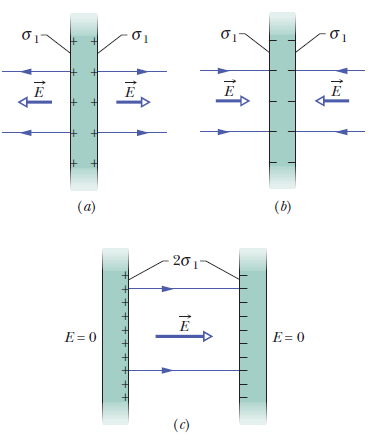
\includegraphics[width=5cm]{Physics2_PNGs/two-conducting-plates.png}
			\caption*{}
			\label{fig:two-conducting-plates.png}
		\end{wrapfigure}
		
		Figure 23-16b shows an identical plate with excess negative charge having the same magnitude of surface charge density $\sigma$. The only difference is that now the electric field is directed toward the plate.
		
		Suppose we arrange for the plates of a and b to be close to each other and parallel. Since the plates are conductors, when we bring them into this arrangement, the excess charge on one plate attracts the excess charge on the other plate, and all the excess charge moves onto the inner faces of the plates as in c. With twice as much charge now on each inner face, the new surface charge density (call it $\sigma_1$) on each inner face is twice $\sigma$. Thus, the electric field at any point between the plates has the magnitude
		
		\begin{equation}
			E = \frac{2\sigma_1}{\varepsilon_0} = \frac{\sigma}{\varepsilon_0}
			\quad \text{(two conducting plates)} \tag{3-13}
		\end{equation}
		
		This field is directed away from the positively charged plate and toward the negatively charged plate. Since no excess charge is left on the outer faces, the electric field to the left and right of the plates is zero.
		


		\subsection*{3.9 Gauss' Law: Spherical Symmetry}
		
		\begin{itemize}
			\item[1.] A shell of uniform charge attracts or repels a charged particle that is outside the shell
			as if all the shell’s charge were concentrated at the center of the shell.  
			\item[2.] If a charged particle is located inside a shell of uniform charge, there is no electrostatic
			force on the particle from the shell.
		\end{itemize}

		We have a charged spherical shell of total charge $q$ and radius $R$, and two concentric spherical Gaussian surfaces ( $S_1$ and $S_2$ ). Applying Gauss’ law to $S_2$ (for which $r \geq R$):
		
		\begin{equation}
			E = \frac{1}{4\pi\varepsilon_0} \frac{q}{r^2}, 
			\tag{(spherical shell, field at $r \geq R$), 3-14}
		\end{equation}
		This field is the same as the one set up by a point charge at the center of the shell. Apllying Gauss' law to $S_1$ (for which $r < R$):
		\begin{equation}
			E = 0,
			\tag{spherical shell, field at $r < R$, 3-15}
		\end{equation}
		Since the surface $S_1$ encloses no charge.
		
		Every distribution with spherical symmetry is a superposition of concentric layers. To apply the two shell theorems, each shell needs to have the same volume charge density $\rho$. Thus for the charge distribution as a whole $\rho$ can only vary with $r$. \\
		Letting $q'$ represent the charge enclosed by any  Gaussian surface, we can
		rewrite Eq. 3-14 as:
		
		\begin{equation}
			E = \frac{1}{4\pi\varepsilon_0} \frac{q'}{r^2},
			\tag{(spherical distribution, field at $r \leq R$), 3-16}
		\end{equation} 
		If the full charge $q$ is uniformly distributed, then $q'$ enclosed within radius $r$ is proportional to $q$:
		
		\[
		\frac{q'}{q} = \frac{\text{volume of sphere } r}{\text{volume of sphere } R}
		\quad \text{or} \quad
		\frac{q'}{\frac{4}{3} \pi r^3} = \frac{q}{\frac{4}{3} \pi R^3} 
		\tag{3-17}
		\]
		This gives us
		\[
		q' = q \frac{r^3}{R^3}
		\tag{3-18}
		\]
		Substituting this into Eq. 3-16 yields:
		\begin{equation*}
			E = \biggl( \frac{q}{4\pi\varepsilon_0 R^3} \biggl) r
			\tag{(uniform charge, field at $r \leq R$), 3-19}
		\end{equation*}
		
		\begin{figure}[h]
			\centering
			\begin{subfigure}{0.45\textwidth} % Adjust width as needed
				\centering
				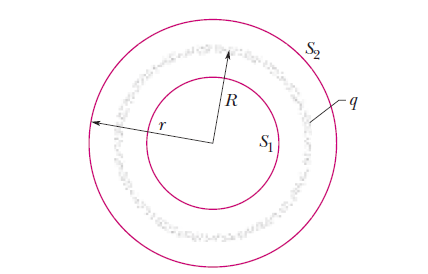
\includegraphics[width=6cm]{Physics2_PNGs/shell-theorem.png} % Replace with actual file
				\caption*{A thin, uniformly charged,
					spherical shell with total charge q, in cross
					section. Two Gaussian surfaces $S_1$ and $S_2$
					are also shown in cross section. Surface $S_2$
					encloses the shell, and $S_1$ encloses only the
					empty interior of the shell.}
				\label{fig:shell-theorem.png}
			\end{subfigure}
			\hfill
			\begin{subfigure}{0.45\textwidth} % Adjust width as needed
				\centering
				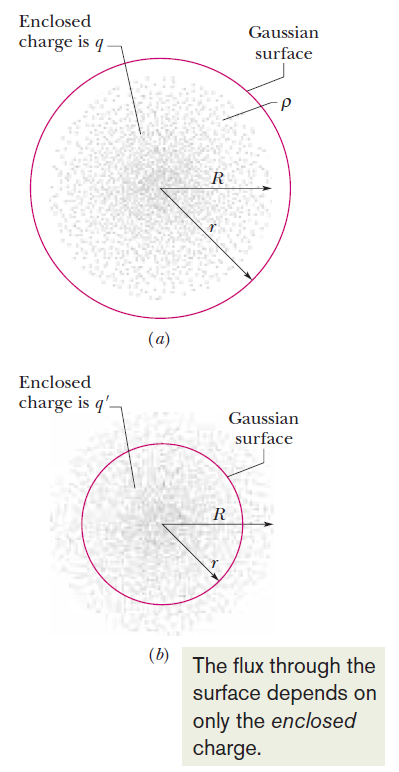
\includegraphics[width=4cm]{Physics2_PNGs/gauss-spherical-symm.png} 
				\caption*{}
				\label{fig:gauss-spherical-symm.png}
			\end{subfigure}
			\caption*{}
			\label{fig:both}
		\end{figure}
		\newpage
		
		
		
		
		\section*{4. Electric Potential}
		
		When an electrostatic force acts between two or more charged particles within a sistem, we can assign an \textbf{electric potential energy} $U$ to the system. If the system changes configuration from an initial state $i$ to a final state $f$, the electrostatic force does work $W$ on the system. We know that the resulting change $\Delta U$ in potential energy is:
	
		\begin{equation*}
			\Delta U = U_f - U_i = -W
			\tag{4-1}
		\end{equation*}
		The potential energy of a charged particle in an electric field varies according to the charge magnitude. However, the potential energy per unit charge [U/q] at any point in the electric field has a singular, definite value and it is called \textbf{electric potential} $V$ at that point (it is also a scalar, not a vector). Thus:
		\begin{equation*}
			V = \frac{U}{q}
			\tag{4-2}
		\end{equation*}
		We can then rewrite the \textit{electric potential difference} $\Delta V$ between two points $i$ and $f$ as:
		\begin{equation*}
			\Delta V = V_f - V_i = \frac{U_f}{q} - \frac{U_i}{q} = \frac{\Delta U}{q}
			\tag{4-3}
		\end{equation*}
		and by substituting $\Delta U =  -W$ we can define the \textit{potential difference} between poin $i$ and $f$ as:
		\begin{equation*}
			\Delta V = V_f - V_i = - \frac{W}{q}
			\tag{potential difference, 4-4}
		\end{equation*}
		By setting $U_f = 0$ at infinity as our reference potential energy, then the potential $V$ must be also 0. Therefore
		\begin{equation*}
			V = - \frac{W_{\infty}}{q}
		\end{equation*}
		The SI unit for potential is joule per coulomb [1 volt = 1 joule / coulomb] and allows us to assign a more conventional unit for electric field $\vec{E}$. By conversion we obtain
		\[
			1 \, N/C = \biggl( 1 \, \frac{N}{C} \biggl) \,
					   \biggl( \frac{1 \, V \cdot C}{1 \, J}\biggl) \,
					   \biggl( \frac{1 \, J}{1 \, N \cdot m} \biggl)
					 = 1 \, V / m
			\tag{4-5}
		\]
		We can also now define another useful unit in the atomic domain: one Electron-Volt (eV) is the energy equal to the work required to move a single elementary charge $e$ through a potential difference of one volt (1 $V$).
		\[
			1 \, \text{eV} = e(1 \text{V}) =  ( 1.60 \cdot 10^{-19} \text{C} )
			( 1 \, \text{J} / \text{C} ) = 1.60 \cdot 10^{-19} \text{J}
		\]
		
		
		
		\subsection*{4.1 Work done by an Applied Force}
		
		We supposedly move a particle of charge $q$ from $i$ to $f$ in an electric field by applying a force to it, this force does work $W_{\text{app}}$ while the electric field does work $W$. By the work-kinetic energy theorem the change in kinetic energy $\Delta K$ of the particle is:
		\begin{equation*}
			\Delta K = K_f - K_i = W_{\text{app}} + W
			\tag{4-6}
		\end{equation*}
		We now suppose the particle is stationary before and after the move. Then $K_f$ and $K_i$ are both zero. There's no change in kinetic energy and Eq.4-6 reduces to:
		\begin{equation*}
			W_{\text{app}} = -W
			\tag{4-7}
		\end{equation*}
		By substituting the latest equation into Eq. 4-1 we find that:
		\begin{equation*}
			\Delta U = U_f - U_i = W_{\text{app}}
			\tag{4-8}
		\end{equation*}
		Doing the same substitution into Eq. 4-4 we find:
		\begin{equation*}
			W_{\text{app}} = q \, \Delta V
			\tag{4-9}
		\end{equation*}
		
		
		
		\subsection*{4.2 Equipotential Surfaces}
		
		Adjacent points with same \textbf{electric potential} form an \textbf{equipotential surface}. While moving a charge between two points of such surface, the electric field does \textit{not} produce work.
		\begin{figure}[!htb]
			\centering
			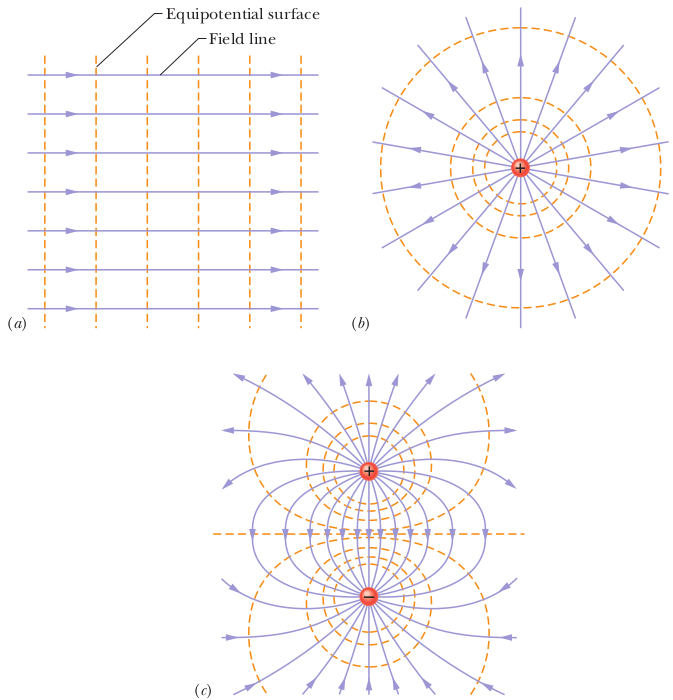
\includegraphics[width=10cm]{Physics2_PNGs/electric-field-lines-surf.png}
			\caption*{}
			\label{fig:electric-field-lines-surf}
		\end{figure} \\
		The work $W$ done by the electric field is zero if the initial and final potentials ($V_f$ and $V_i$) are the same.
		This zero work condition holds for any path connecting two points on the same equipotential surface. \\ 
		- Equipotential surfaces for a point charge or spherically symmetric charge  distribution are \textbf{concentric spheres}. \\
		- For a uniform electric field, these surfaces are \textbf{planes} \textit{perpendicular} to the field lines. \\
		Electric field ($\vec{E}$) lines are always perpendicular to equipotential surfaces. If $\vec{E}$ was not perpendicular, it would do work on a charged particle moving along the surface, which contradicts the definition of an equipotential surface. \\ \\
		Therefore, since any movement along the surface has $W = 0$, we can say:
		\[
			W = \vec{F} \cdot \vec{d} = q \, \vec{E} \cdot \vec{d}
			  = q \, E \, d \, \cos \theta = 0 \rightarrow \theta = 90\text{°} \quad \text{(perpendicular)}
		\]
		
		
		
		\subsection*{4.3 Calculating the Potential from the Electric Field}
		
		Considering an arbitrary electric field $\vec{E}$ and a positive test charge $q_0$ moving from two points $i$ and $f$ in the field. At any point in the path an electrostatic force $q_0 \, \vec{E}$ acts on the charge as it moves through a differential displacement $d\vec{s}$. We know that:
		\[
			dW = \vec{F} \cdot d\vec{s}
			\tag{4-10}
		\]
		Given that $\vec{F} = q_0 \, d\vec{s}$ Eq. 4-10 becomes:
		\[
			dW = q_0 \vec{E} \cdot d\vec{s}
			\tag{4-11}
		\]
		To find the total work $W$ done on the particle as it moves from $i$ to $f$ we sum the differential work through all the displacements $d\vec{s}$:
		\begin{equation*}
			W = q_0 \int_{i}^{f} \vec{E} \cdot d\vec{s}
			\tag{4-12}
		\end{equation*}
		Or, in terms of potential difference
		\begin{equation*}
			V_f - V_i = - \int_{i}^{f} \vec{E} \cdot d\vec{s}
			\tag{4-13}
		\end{equation*}
		This yield the same result since the electrostatic force is \textit{conserative} and every path returns the same result. If we set $V_i = 0$, Eq. 4-13 becomes:
		\begin{equation*}
			V = - \int_{i}^{f} \vec{E} \cdot d\vec{s}
			\tag{4-14}
		\end{equation*}
		giving us the potential $V$ at any final point $f$ in the electric field, relative to the \textit{zero} potential in the initial point. \\
		
		In pratical terms, if we let $i$ be at infinity, Eq.4-14 gives us the potential $V$ at any point $f$.
		
		
		
		\subsection*{4.4 Potential due to a Point Charge}
	
		\begin{wrapfigure}{r}{0.19\textwidth}
			\centering
			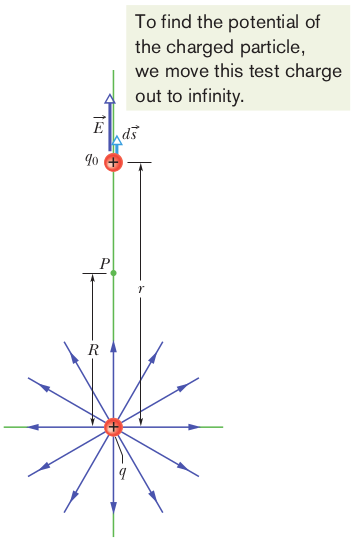
\includegraphics[width=5.5cm]{Physics2_PNGs/point-charge-potential.png}
			\caption*{}
			\label{fig:point-charge-potential.png}
		\end{wrapfigure}
		We need to find an expression to intercept the electric potential $V$ relative to the zero potential at infinity. Considering a point $P$ at a distance $R$ from a  positive point charge $q$ we can use Eq. 4-13 to achieve such task. Let us first evaluate the dot product: 
		\begin{equation*}
			\vec{E} \cdot d\vec{s} = E \, \cos\theta \, ds
			\tag{4-15}
		\end{equation*}
		Since the electric field $\vec{E}$ is directed radially outward from the particle the differential displacement $d\vec{s}$ has same direction as $\vec{E}$. That means that in Eq. 4-15, $\theta = 0$ and $\cos\theta = 1$ accordingly. Given that the path is radial we can write $ds$ as $dr$ and we can evaluate Eq. 4-13 from $R$ to $\infty$:
		\begin{equation}
			V_f - V_i = - \int_{R}^{\infty} E \, dr
			\tag{4-16}
		\end{equation}
		We now set $V_f = 0 \, ( \text{at} \, \infty )$ and $V_i = V$, we also know that the magnitude $E$ is equal to:
		\[
			E = \frac{1}{4 \pi \varepsilon_0} \, \frac{q}{r^2}
		\]
		With these informations, 4-16 becomes:
		\begin{equation*}
			0 - V = - \frac{q}{4 \pi \varepsilon_0} \int_{R}^{\infty} \frac{1}{r^2} \, dr
				  = \frac{q}{r \pi \varepsilon_0} \biggl[ \frac{1}{r} \biggl]_R^\infty
				  = - \frac{1}{4 \pi \varepsilon_0} \frac{q}{R}
			\tag{4-17}
		\end{equation*}
		Solving for $V$ and substituting $R$ with $r$:
		\begin{equation*}
			V = \frac{1}{4 \pi \varepsilon_0} \frac{q}{r}
			\tag{Potential due to Point Charge, 4-18}
		\end{equation*}
		A positively charged particle produces a positive electric potential. A negatively
		charged particle produces a negative electric potential. 
		
		We can also prove, using the shell theorems, that this expression is also valid for \textit{spherical charge distributions}.



		\subsection*{4.5 Potential due to Group of Point Charges}

		The superposition principle holds for electric potential $V$ as well, therefore, for $n$ charges, the net potential will be: 
		\begin{equation*}
			V = \sum_{i=1}^{n} V_i 
			  = \frac{1}{4 \pi \varepsilon_0} \sum_{i=1}^{n} \frac{q_i}{r_i}
			  \tag{Potential due to $n$ point charges, 4-19}
		\end{equation*}



		\subsection*{4.6 Potential due to an Electric Dipole}

		\begin{wrapfigure}{r}{0.1\textwidth}
			\centering
			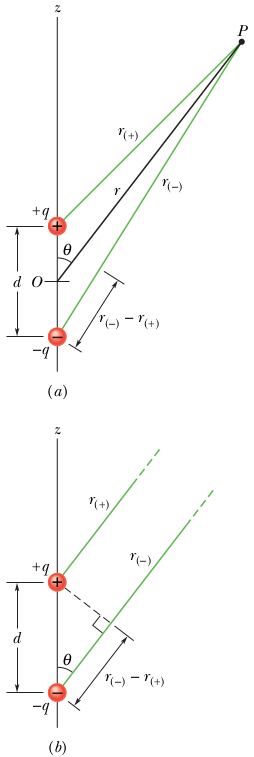
\includegraphics[width=3.25cm]{Physics2_PNGs/dipole-point-potential.png}
			\caption*{}
			\label{fig:dipole-point-potential.png}
		\end{wrapfigure}

		Now let's apply 4-19 to an electric dipole to find the potential at any arbitrary point $P$, in which the positive point charge ( at distance $r_{(+)}$ ) sets up potential $V_{(+)}$ and the negative charge sets $V_{(-)}$ at distance $r_{(-)}$. \\	Therefore the net potential is given by:
		\begin{equation*}
			V = \sum_{i=1}^{2} V_i = V_{(+)} + V_{(-)}
			  = \frac{1}{4 \pi \varepsilon_0} \biggl( \frac{q}{r_{(+)}} + 
			  										  \frac{-q}{r_{(-)}} \biggl)
			  =  \frac{q}{4 \pi \varepsilon_0} \frac{r_{(-)} - r_{(+)}}{r_{(+)}r_{(-)}}
			  \tag{4-20}
		\end{equation*}
		Since we're interested in points far from the dipole, such as $r \gg d$, where $d$ is the distance between the charges, we can approximate
		\[
			r_{(+)} - r_{(-)} \approx d \cos\theta 
			 \quad \text{and} \quad r_{(+)} r_{(-)} \approx r^2
		\]
		By substituting these quantities into Eq. 4-20 we can approximate $V$ to be:
		\[
			V = \frac{q}{4 \pi \varepsilon_0} \frac{d \, \cos \theta}{r^2}
		\]
		where $\theta$ is measured from the dipole axis. We can then express V as:
		\begin{equation*}
			V = \frac{1}{4 \pi \varepsilon_0} \frac{p \cos \theta}{r^2}
			\tag{Electric Dipole, 4-21}
		\end{equation*}
		in which $p$ ($=q\,d$) is the magnitude of the electric dipole moment vector $\vec{p}$, directed along the dipole axis (meaning $\theta$ is measured from the direction of $\vec{p}$).



	%	\newpage
		
		\subsection*{4.7 Potential Due to a Continous Charge Distribution}

		When a charge $q$ is continous we must choose a differential $dq$, determine the potential $dV$ at $P$ due to $dq$ and then integrate over the entire distribution. 
		If we take the \textit{zero} potential at infinity and treat $dq$ as a point charge: 
		\begin{equation*}
			dV = \frac{1}{4 \pi \varepsilon_0} \frac{dq}{r} 
			\tag{4-22}
		\end{equation*}
		$dq$ can be either negative or positive. The total potential $V$ at $P$ is then given by the sum of every differential $dq$, obtained via integration:
		\begin{equation}
			V = \int dV = \frac{1}{4 \pi \varepsilon_0} \int \frac{dq}{r}
			\tag{Continous Charge Distribution, 4-23}
		\end{equation}
	
	
	
		\subsection*{4.7.1 Continous Distributions: Line of Charge}
		
		\begin{wrapfigure}{r}{0.17\textwidth}
			\centering
			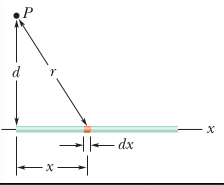
\includegraphics[width=5cm]{Physics2_PNGs/rod-continous.png}
			\caption*{}
			\label{fig:rod-continous.png}
		\end{wrapfigure}
		Thin, nonconducing rod of length $L$ with positive charge of uniform linear density $\lambda$. Let's determine the potential $V$ due to the rod at a point $P$ with perpendicular distance $d$ from the left end of the rod. We consider a differential element $dx$ of the rod. This element has differential charge of:
		\[
			dq = \lambda \, dx
			\tag{4-24}
		\]
		This element produces an electric potential $dV$ at $P$, which has distance 
		$r = (x^2 + d^2)^{1/2}$ from $dx$. Treating this element as a point charge, we can use Eq. 4-22 to write $dV$ as:
		\begin{equation*}
			dV = \frac{1}{4 \pi \varepsilon_0} \frac{dq}{r}
			   = \frac{1}{4 \pi \varepsilon_0} \, \frac{\lambda \, dx}{(x^2 + d^2)^{1/2}}
			\tag{4-25}
		\end{equation*}
		Since the charge on the rod is positive and we have taken $V = 0$ at infinity, then $dV$ must be positive. \\
		We can now find $V$ by integrating along the length of the rod, from $x = 0$ to 
		$x = L$:
		\begin{equation*}
			V = \int dV = \int_{0}^{L} \frac{1}{4 \pi \varepsilon_0}
			              \, \frac{\lambda}{(x^2 + d^2)^{1/2}} \, dx 
		\end{equation*}
		\[
			= \frac{\lambda}{4 \pi \varepsilon_0} \, 
			  \int_0^L \frac{\lambda}{(x^2 + d^2)^{1/2}} \, dx
		\]
		\[
			= \frac{\lambda}{4 \pi \varepsilon_0} 
			    \biggl[ \ln \biggl( x + (x^2 + d^2)^{1/2} \biggl) \biggl]_0^L
		\]
		\[
			= \frac{\lambda}{4 \pi \varepsilon_0} 
				\biggl[ \ln \biggl( L + (L^2 + d^2)^{1/2} \biggl) - \ln d \, \biggl]
		\]
		
		We can further simplify the expression by using the relation $\ln A - \ln B = \ln ( A / B )$. Hence we can write: 
		\begin{equation*}
			V = \frac{\lambda}{4 \pi \varepsilon_0} 
			     \ln \biggl[ \frac{L + ( L^2 + d^2 )^{1/2}}{d} \biggl]
			\tag{Potential due to Line of Charge, 4-26}
		\end{equation*}
		$V$ will be as a result positive, being it a sum of positive values of $dV$, being also consistent with the logarithm being positive with values bigger than 1 in the argument. 
		
		
	%	\newpage
		
		\subsection*{4.7.2 Continous Distributions: Charged Disk}

		\begin{wrapfigure}{r}{0.17\textwidth}
			\centering
			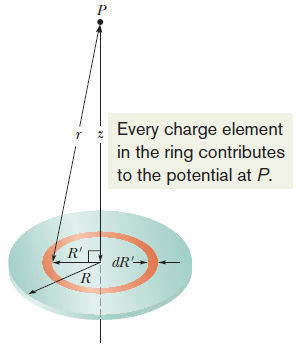
\includegraphics[width=4.5cm]{Physics2_PNGs/disk-continous.png}
			\caption*{}
			\label{fig:disk-continous.png}
		\end{wrapfigure}
		Plastic disk of radius $R$ that has a uniform charge density $\sigma$ on one surface. We need to derive an expression for $V(z)$, the electric potential at any point on the central axis.
		
		Consider a differential element consisting of a flat ring of radius \( R' \) and radial width \( dR' \). Its charge has magnitude:
		\[
		dq = \sigma (2\pi R') (dR'),
		\]
		in which $(2\pi R')(dR')$ is the upper surface area of the ring. All parts of this charged element are the same distance $r$ from point $P$ on the disk’s axis. We can use Eq. 4-22 to write the contribution of this ring to the electric potential at \( P \) as
		
		\[
			dV = \frac{1}{4\pi \epsilon_0} \frac{dq}{r} = \frac{1}{4\pi \epsilon_0} 		 \frac{\sigma (2\pi R')(dR')}{\sqrt{z^2 + R'^2}}
			\tag{4-27}
		\]
		We find the net potential at $P$ by integrating the contributions of all the rings from $R' = 0$ to $R' = R$:
		
		\[
			V = \int dV = \frac{\sigma}{2\epsilon_0} \int_0^R \frac{R' \, dR'}{\sqrt{z^2 + R'^2}} = \frac{\sigma}{2\epsilon_0} (\sqrt{z^2 + R^2} - z)
			\tag{Charged Disk, 4-28}
		\]
		Also the variable in the second integral in 4-28 is $R'$ and not $z$, which remains constant.
		\\\\\\
		
		
	%	\newpage
		
		
		\subsection*{4.8 Calculating Field ($\vec{E}$) from the potential ($V$)}

		\begin{wrapfigure}{r}{0.17\textwidth}
			\centering
			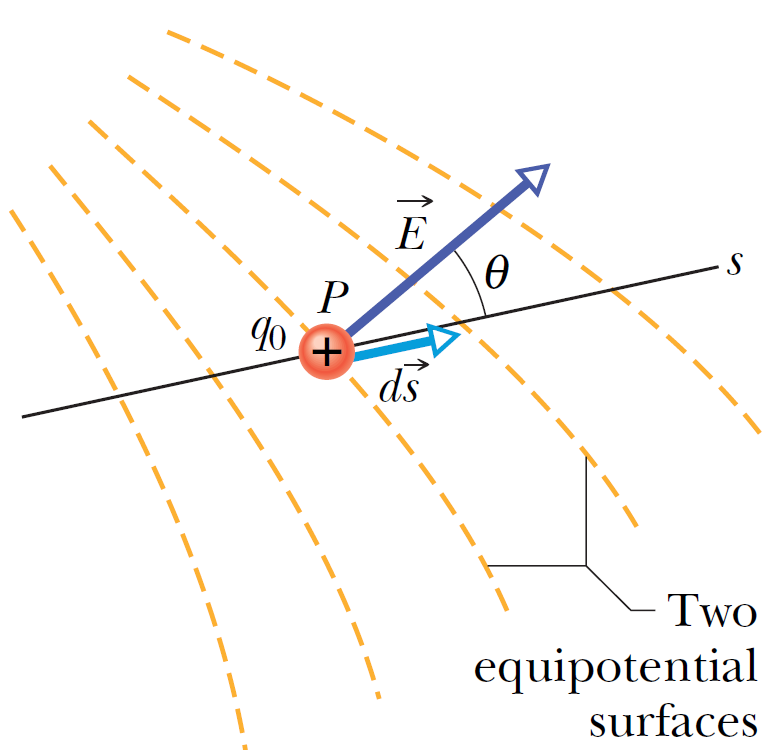
\includegraphics[width=4.5cm]{Physics2_PNGs/charge-in-elec-field.png}
			\caption*{}
			\label{fig:charge-in-elec-field.png}
		\end{wrapfigure}
		We can find the potential $V$ from the Field $\vec{E}$ by using \\ 
		$V_f - V_i = - \int_{i}^{f} \vec{E} \cdot d\vec{s}$. We can easily search for the field $\vec{E}$ from the potential $v$ by looking at it graphically. $\vec{E}$ is perpendicular to the equipotential surface, with intensity inversely proportional to distance $d\vec{s}$. We must then move $q_0$ on a by a differential distance $d\vec{s}$. From Eq. 4-4 we see that the work done on the charge is $-q_0 \, dV$, while from Eq. 4-11 we get that the work done by the field can be written as $(q_0\vec{E}) \cdot d\vec{s}$, or $q_0E(\cos\theta)  \, ds$. \\
		Equating these expression for work yields:
		\[
			-q_0 \, dV = q_0E(\cos\theta) \, ds
			\tag{4-29}
		\]
		or
		\[
			E \, \cos\theta = - \frac{dV}{ds}
			\tag{4-30}
		\]
		Since $E$ is dependant on variation oon different axis (in this case the $s$ axis), we rewrite 4-30 as:
		\begin{equation*}
			E_s = - \frac{\partial V}{\partial s}
			\tag{4-31}
		\end{equation*}
		Rewriting in a general form, involving space coordinates:
		\begin{equation*}
			E_x = - \frac{\partial V}{\partial x}; \quad
			E_y = - \frac{\partial V}{\partial y}; \quad
			E_z = - \frac{\partial V}{\partial z}.
			\tag{4-32}
		\end{equation*}



		\subsection*{4-9 Electric Potential Energy of a System of Point Charges}

		\begin{wrapfigure}{r}{0.17\textwidth}
			\centering
			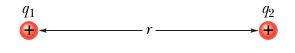
\includegraphics[width=4.5cm]{Physics2_PNGs/2-charges-potential.png}
			\caption*{}
			\label{fig:2-charges-potential.png}
		\end{wrapfigure}
		The electric potential energy of a system of fixed point charges is equal to \textit{the work that must be done by an external agent to assemble the system}, bringing each charge in from an infinite distance. \\
		We assume the simplest case, a system of 2 charges $q_1$ and $q_2$, separated by a change $r$. We can consider the work done and drop the minus sign in Eq. 4-4 since we're only interested in the work actually done, instead of the work done by the field. Therefore in our case the work done will be equal to $q_2V$, where $V$ is the potential set up by $q_1$ at the point where $q_2$ stands. \\
		From Eq. 4-18 the potential then becomes:
		\[
			V = \frac{1}{4 \pi \varepsilon_0} \frac{q_1}{r}
		\]
		Therefore the electric potential energy from the pair of point charges is:
		\begin{equation*}
			U = W = q_2 V = \frac{1}{4 \pi \varepsilon_0} \frac{q_1 q_2}{r}
			\tag{4-33}
		\end{equation*}
		If the charges have same sign, we have to do positive work to push them together against their own repulsion, the potential energy of the system is then \textit{positive}. \\
		If the charges have opposite sign, we will have to do negative work to keep them stationary, therefore the potential energy of the system will be \textit{negative}.



		\subsection*{4.10 Potential of a Charged Isolated Conductor}
		
		\begin{wrapfigure}{r}{0.17\textwidth}
			\centering
			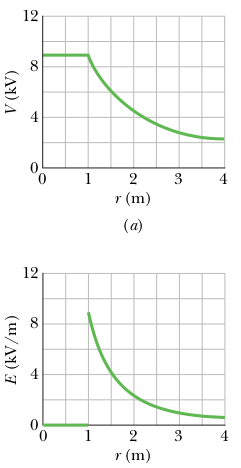
\includegraphics[width=3.5cm]{Physics2_PNGs/plot-charge-potential.png}
			\caption*{}
			\label{fig:plot-charge-potential.png}
		\end{wrapfigure}
		We know that $\vec{E} = 0$ for all points inside an isolated conductor and that an excess charge placed on it lies entirely on its surface. We also can extend this definition to say that all the points in the conductor will come to the same potential. And that's true even if the conductor has any kind of internal cavity and also if there's a net charge inside said cavity. 6Therefore:
		\begin{equation*}
			V_f - V_i = - \int_{i}^{f} \vec{E} \cdot d\vec{s}
		\end{equation*}
		Since $\vec{E} = 0$ it is a	consequence that $V_f - V_i = 0$, thus $V_f = V_i$ for every pair of point $i$ and $f$ in the conductor. \\
		Let's take for example a \textit{spherical isolated	conducting shell} of radius $r = 1.0$ m, having charge $q = 1.0$ $\mu$C. \\
		From Eq. 4-18 we can calculate how $V(r)$ behaves as if it were concentrated at the center of the shell for external points. If we push a charge through the shell in its center (assuming such small hole exists) no extra work is needed since no net electric force acts on the charge. \\ \\
		We can therefore say that, for every point inside the shell, the potential $V$ is constant and the field $E = 0$. \\
		On the outside, instead,  we have 
		\[
			V = \frac{q}{4 \pi \varepsilon_0 r'}, \quad \quad
			E = - \frac{dV}{dr} = \frac{q}{4 \pi \varepsilon_0 r^2}
		\]
		The plot shows the result of these considerations.
		
		
		
		\subsection*{4.10.1 Isolated Conductor in an Electric Field}

		\begin{wrapfigure}{r}{0.17\textwidth}
			\centering
			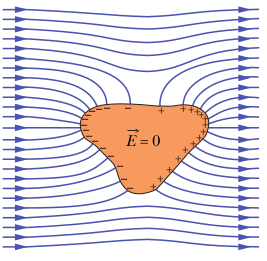
\includegraphics[width=4.2cm]{Physics2_PNGs/isolated-conduct-elec-field.png}
			\caption*{}
			\label{fig:isolated-conduct-elec-field.png}
		\end{wrapfigure}
		If an \textit{isolated conductor} is placed in an \textit{external electric field}, all points of the conductor still come to a single potential regardless of whether the conductor has excess charge. \\
		The \textit{free conduction electrons} distribute themselves on the surface such that the electric field they produce at interior points cancel the external electric field that would be there otherwise.  \\
		The electron distribution would cause the net electric field at all points on the surface to be perpendicular to the surface itself. \\
		In brief, the free electrons in the conductor will distribute themself over the surface, leaving the electric field $E = 0$.
		
		
		
		
		\newpage
		
		\section*{5. Capacitance}
		
		The \textbf{Capacitor} is a device capable of \textit{storing} electrical energy. \\
		Its physics can be generalized to other devices or situations, for example, Earth's atmospheric electric field has same properties as a spherical capacitor. \\
		The amount of electrical energy that a capacitor can store is called 
		\textbf{capacitance}.\\
		\begin{wrapfigure}{r}{0.17\textwidth}
			\centering
			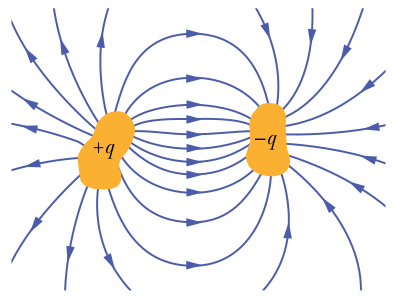
\includegraphics[width=4.2cm]{Physics2_PNGs/capacitor-scheme.png}
			\caption*{}
			\label{fig:capacitor-scheme.png}
		\end{wrapfigure}
		The basic elements of any capacitor are two isolated conductors that we call \textit{plates} regardless of their geometry. \\
		A capacitor is \textit{charged} if its plates have have charges of equal magnitude but opposite signs: $+q$ and $-q$. However we refer to the charge of the capacitor as $q$, being it the absolute value of the charges on the plates (also $q$ is not the net charge, which is \textit{zero}). \\
		There is a potential difference between the two plates, which, for historical reason, which value we refer to as $V$ in behalf of $\Delta V$. \\
		The charge $q$ and the potential difference $V$ are proportional to each other 
		($q \propto V$):
		\begin{equation*}
			q = CV
			\tag{5-1}
		\end{equation*}
		In which the constant $C$ is called \textbf{capacitance} of the capacitor.
		
		The SI unit of capacitance is the coulomb per volt, referred to as \textit{farad} (F):
		\[
			1 \, \text{farad} = 1 \, \text{F} = 1 \, \text{coulomb per volt} = 1 \,
			\text{C} / \text{V}
			\tag{5-2}
		\]
		Usually in pratical applications, submultiples of the farad are more common \\
		1 mF $= 10^{-3}$ F \\ 1 $\mu$F $= 10^{-6}$ F \\ 
		1 nF $= 10^{-9}$ F \\ 1 pF $= 10^{-12}$ F		
		
		
		\subsection*{5.1 Charging a Capacitor}
		
		\begin{wrapfigure}{r}{0.37\textwidth}
			\centering
			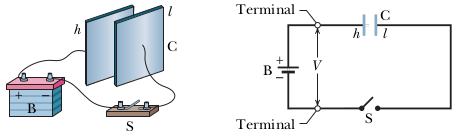
\includegraphics[width=8cm]{Physics2_PNGs/capacitor-charging.png}
			\caption*{}
			\label{fig:capacitor-charging.png}
		\end{wrapfigure}
		One way to charge a capacitor is to place it in a circuit with a \textit{battery} \\
		In the figure, a battery \textbf{B}, a switch \textbf{S}, an uncharged capacitor \textbf{C} and interconnecting wires form a circuit. \\
		The battery mantains a potential difference $V$ between its terminal, in which the positive terminal, with higher potential, is labeled + and the negative terminal, with lower potential, is labeled --. \\
		When the switch S is open the circuit is said to be \textit{incomplete} (since the components aren't electrically connected and charge can't flow). If the switch is closed then the circuit is \textit{complete}. \\
		When the plates of the capacitor are uncharged, its potential is \textit{zero}. As we close the switch S, the capacitor C begins to charge until its plates match the potential $V$ between the terminals in the battery. The capacitor is then said to be \textit{fully charged}. 
		
		
		
		\newpage
		
		\subsection*{5.2 Calculating Capacitance}
		
		The goal it's to calculate the capacitance of a capacitor once the geometry is known. In brief: (1) Assume charges $+q$ and $-q$ on the plates, (2) calculate electric field $\vec{E}$ between the plates in term of said charge, using Gauss' Law, (3) knowing $\vec{E}$ calculate potential $V$ between the plates, (4) calculate C using Eq. 5-1.
		
		\subsection*{5.2.1 Calculating Capacitance: Electric Field}
		
		To relate electric field $\vec{E}$ between platess of the capacitor on the charge $q$ on either plate, we use Gauss' Law:
		\begin{equation*}
			\varepsilon_0 \oint \vec{E} \cdot d\vec{A} = q
			\tag{5-3}
		\end{equation*}
		We consider a gaussian surface such that $\vec{E}$ has uniform magnitude $E$ and vectos $\vec{E}$ and $\vec{A}$ will be parallel. 5-3 then reduces to:
		\begin{equation*}
			q = \varepsilon_0 E A 
			\tag{5-4}
		\end{equation*}
			
		\subsection*{5.2.2 Calculating Capacitance: Potential Difference}
		
		From Eq. 4-13 we know the potential difference between the plates of a capacitor is related to the field $\vec{E}$:
		\begin{equation*}
			V_f - V_i = - \int_{i}^{f} \vec{E} \cdot d\vec{A}
			\tag{5-5}
		\end{equation*}
		in which the integral is evaluated along any path that starts on one plate and ends on the other. We choose a path that follows an electric field line, from negative (--) to positive (+) plate. For such path, $\vec{E} \cdot d\vec{A} = -E \, ds$. Letting $V = V_f - V_i$:
		\begin{equation*}
			V = \int_{-}^{+} E \, ds
			\tag{5-6}
		\end{equation*}
		
		
		
		\subsection*{5.2.3 Parallel-Plate Capacitor}
			
		\begin{wrapfigure}{r}{0.37\textwidth}
			\centering
			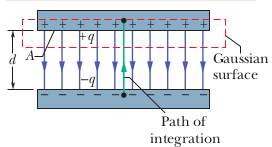
\includegraphics[width=5cm]{Physics2_PNGs/capacitor-charging-closeup.png}
			\caption*{}
			\label{fig:capacitor-charging-closeup.png}
		\end{wrapfigure}
		We assume that the plates of our parallel-plate capacitor are so large and so close together that we can neglect the fringing of the electric field at the edges of the plates. \\
		We draw a Gaussian surface that encloses just $q$ on the positive plate. From Eq. 5-4 we can write:
		\begin{equation*}
			q = \varepsilon_0 EA
			\tag{5-7}
		\end{equation*}
		Where A is the area of the plate. \\
		Eq. 5-6 yields:
		\begin{equation*}
			V = \int_{-}^{+} E \, ds = E \int_{0}^{d} ds = Ed
			\tag{5-8}
		\end{equation*}
		In which $d$ is just the plate separation distance. \\
		If we now substitute $q$ from Eq. 5-7 and $V$ from Eq. 5-8 into the relation $q = CV$ (Eq. 5-1):
		\[
				C = \frac{\varepsilon_0 A}{d}
				\tag{Parallel-Plate Capacitor, 5-9}
		\]
		This result allows us to express in a different way for problems involving capacitor, namely:
		\[
			\varepsilon_0 = 8.85 \cdot 10^{-12} \, \text{C}^2 / \text{N} \cdot \text{m}^2
						  = 8.85 \cdot 10^{-12} \, \text{F/m} = 8.85 \, \text{pF/m}
			\tag{5-10}
		\]



		\subsection*{5.2.4 Cylindrical Capacitor}

		\begin{wrapfigure}{r}{0.37\textwidth}
			\centering
			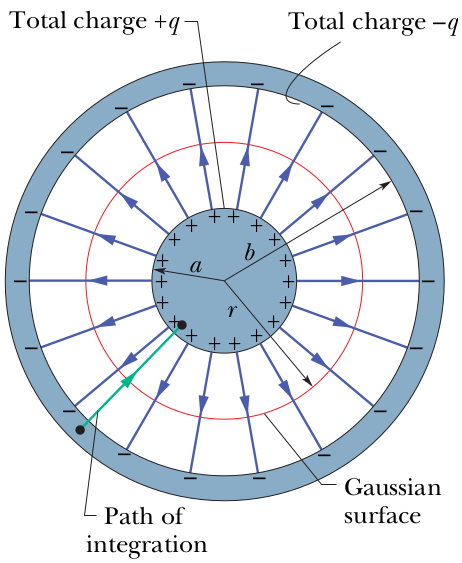
\includegraphics[width=5cm]{Physics2_PNGs/cylindrical-capacitor.png}
			\caption*{}
			\label{fig:cylindrical-capacitor.png}
		\end{wrapfigure}
		As in figure, we have a cylindrical capacitor of length $L$ formed by two coaxial cylinders of radii $a$ and $b$. We assume $L \gg b$ so that we can neglect the fringing of the electric field that occurs at the ends of the cylinders. Each plate contains charge of magnitude $q$. \\
		We choose a cylinder of length $L$ and radius $r$ as gaussian surface, coaxial with the cylinders and placed such that it encloses the central cylinder and its charge $q$. By relating charge and field magnitude $E$ with Eq. 5-4:
		\[
			q = \varepsilon_0 E A = \varepsilon_0 E (2 \pi r L)
		\]
		in which $2 \pi r L$ is the area of the curved part of the gaussian surface. There is no flux through end caps, therefore:
		\[
			E = \frac{q}{2 \pi \varepsilon_0 L r}
			\tag{5-11}
		\]
		substituting into 5-6 yields:
		\[
			V = \int_{-}^{+} E ds 
			  = - \frac{q}{2 \pi \varepsilon_0 L} \int_{b}^{a} \frac{dr}{r}
			  = \frac{q}{2 \pi \varepsilon_0 L} \ln \frac{b}{a}  
			  \tag{5-12}
		\]
		where we used $ds = -dr$ (we integrated radially). \\
		From the relation $C = qV$:
		\begin{equation*}
			C = 2 \pi \varepsilon_0 \, \frac{L}{\ln (b/a)}
			\tag{Cylindrical Capacitor, 5-13}
		\end{equation*}
		
		
		
		\subsection*{5.2.5 Spherical Capacitor}
		
		Capacitor consisting of two concentric spherical shells, of radii $a$ and $b$. As gaussian surface we draw a sphere of radius $r$ concentric with the two shells, Eq. 5-4 yields:
		\begin{equation*}
			q = \varepsilon_0 E A = \varepsilon_0 E (4 \pi r^2)
		\end{equation*}
		in which $(4 \pi r^2)$ is the area of the spherical gaussian surface. By solving the equation for E we obtain:
		\begin{equation*}
			E = \frac{1}{4 \pi \varepsilon_0} \frac{q}{r^2}
			\tag{5-14}
		\end{equation*}
		which is the electric field due to an uniform spherical distribution. By substituting into Eq. 5-6:
		\begin{equation*}
			V = \int_{-}^{+} E ds 
			  = - \frac{q}{4 \pi \varepsilon_0} \int_{b}^{a} \frac{dr}{r^2} 
			  = \frac{q}{4 \pi \varepsilon_0} \biggl( \frac{1}{a} - \frac{1}{b} \biggl)
				  = \frac{q}{4 \pi \varepsilon_0} \frac{b - a}{ab}
			\tag{5-15}
		\end{equation*}		
		where, again, $ds = -dr$. By substituting into Eq. 5-1 and solving for capacitance C:
		\begin{equation*}
			C = 4 \pi \varepsilon_0 \, \frac{ab}{b - a} 
			\tag{Spherical Capacitor, 5-16}
		\end{equation*}
	
	
		
		\subsection*{5.2.6 Isolated Sphere}
		
		We can assign a capacitance to a single isolated spherical conductor of radius $R$
		by assuming that the “missing plate” is a conducting sphere of infinite radius.
		To find the capacitance of the conductor we rewrite 5-16 as:
		\[
			C = 4 \pi \varepsilon_0 \, \frac{a}{1 - a/b}
		\]
		by letting $b \rightarrow \infty$ and substituting $R$ for $a$, we find:
		\[
			C = 4 \pi \varepsilon_0 R
			\tag{Isolated Sphere, 5-17}
		\]
		
		\subsection*{5.3 Capacitors in Parallel and in Series}
		
		When there's a combination of capacitors in a circuit, we can replace that combination with an \textbf{equivalent capacitor}, useful to simplify the circuit.
		
		\subsection*{5.3.1 Capacitors in Parallel}
		
		\begin{wrapfigure}{r}{0.26\textwidth}
			\centering
			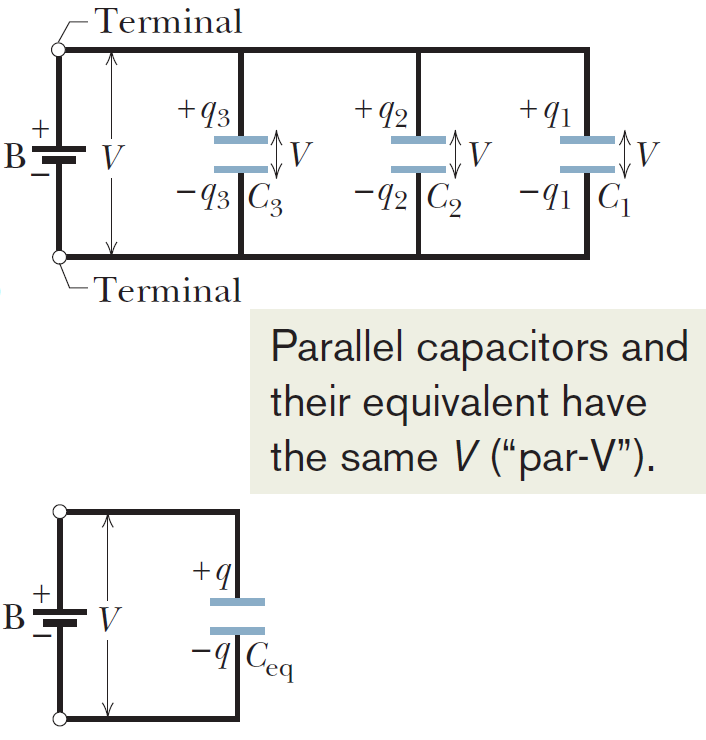
\includegraphics[width=6.5cm]{Physics2_PNGs/parallel-capacitors.png}
			\caption*{}
			\label{fig:parallel-capacitors.png}
		\end{wrapfigure}
		When a potential difference $V$ is applied across several capacitors connected in parallel, it is applied through each capacitor. The total charge $q$ stored on the capacitors is the sum of the charges stored in each capacitor.\\
		Therefore we can replace the capacitors connected in parallel with an equivalent capacitor that has the same total charge q and same potential difference $V$ as the actual capacitors. \\
		We can derive an expression for $C_{eq}$ by finding the charge on each actual capacitor, given 3 parallel capacitors($q_1$, $q_2$, $q_3$):
		\[
			q_1 = C_1 V, \quad q_2 = C_2 V, \quad q_3 = C_3 V
		\]
		The total charge on the parallel is then:
		\[
			q = q_1 + q_2 + q_3 = (C_1 + C_2 + C_3)V
		\]
		The equivalent capacitance, with same total charge $q$ and applied potential difference $V$ is then:
		\[
			C_{eq} = \frac{q}{V} = C_1 + C_2 + C_3
		\]
		Extending this result to any number $n$ of capacitors:
		\begin{equation*}
			C_{eq} = \sum_{j=1}^{n} C_j
			\tag{$n$ Capacitors in Parallel, 5-18}
		\end{equation*}
		
		
		
		\newpage
		
		\subsection*{5.3.2 Capacitors in Series}
		
		\begin{wrapfigure}{r}{0.2\textwidth}
			\centering
			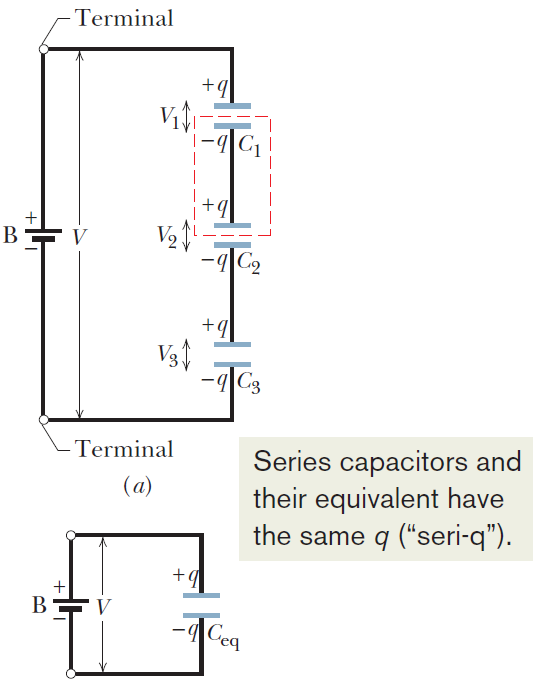
\includegraphics[width=5.5cm]{Physics2_PNGs/series-capacitors.png}
			\caption*{}
			\label{fig:series-capacitors.png}
		\end{wrapfigure}
		When a potential difference $V$ is applied through several capacitors connected in series, the capacitors have identical charge $q$. The sum of the potential differences across all the capacitors is equal to the applied potential difference $V$. \\
		Therefore they can be replaced with an equivalent capacitor that has the same charge $q$ and same total potential difference $V$ as the actual series capacitors.
		We can derive an expression for $C_{eq}$ by finding the potential difference on each capacitor:
		\[
			V_1 = \frac{q}{C_1}, \quad V_2 = \frac{q}{C_2}, \quad V_3 = \frac{q}{C_3}
		\]
		The total potential difference $V$ due to the battery is the sum  of these three potential differences. Thus:
		\[
			V = V_1 + V_2 + V_3 = q \, \biggl( 
				\frac{1}{C_1} + \frac{1}{C_2} + \frac{1}{C_3} \biggl)
		\]
		The equivalent capacitance is then
		\[
			C_{eq} = \frac{q}{V} = \frac{1}{1/C_1 + 1/C_2 + 1/C_3}
			\quad \text{or} \quad
			\frac{1}{C_{eq}} = \frac{1}{C_1} + \frac{1}{C_2} + \frac{1}{C_3}	
		\]
		We can generalize to any number $n$ of capacitor as:
		\begin{equation*}
			\frac{1}{c_{eq}} = \sum_{j=1}^{n} \frac{1}{C_j}
			\tag{$n$ Capacitors in Serier, 5-19}
		\end{equation*}
		
		
		
		\subsection*{5.4 Energy Stored in an Electric Field}

		
		In order to charge a capacitor, work must be done by an external agent. We can visualize the work required to charge a capacitor as being stored in form of potential energy $U$ in the electrif field between the plates. The energy can be recovered in any moment, by discharging the capacitor. \\
		Suppose that at any given instant, a charge $q'$ has been transferred to one plate to the other. The potential difference $V'$ between the plate at that instant will be $q'/C$. If an increment of charge $dq'$ is transferred, the increment in work will be:
		\[
			dW = V' \, dq' = \frac{q'}{C} \, dq'
		\]
		The work required to totally charge up the capacitor to a final value $q$ is then:
		\[
			W = \int dW = \frac{1}{C} \int_{0}^{q} q' \, dq' = \frac{q^2}{2C}
		\]
		which is stored as \textit{potential energy} $U$ in the capacitor, therefore:
		\begin{equation*}
			U = \frac{q^2}{2C}
			\tag{Potential Energy, 5-20}
		\end{equation*}
		From 5-1 we can also write this as:
		\begin{equation*}
			U = \frac{1}{2} CV^2
			\tag{Potential Energy, 5-21}
		\end{equation*}
		These equations hold regardless of the geometry of the capacitor. \\ \\
		In brief: the potential energy $V$ of a charged capacitor $C$ can be viewed as being stored in the electric field between the plates.
		
		
		\subsection*{5.4.1 Energy Density}
		
		Considering a parallel-plate capacitor, neglecting fringing, the electric field has same value at all points between the plates. Thus the \textbf{energy density} $u$ (potential energy per unit volume between the plates) should also be uniform. \\
		We can find $u$ by dividing the total potential energy by the volume $Ad$ of the space between the plates. By using Eq. 5-21 we yield:
		\[
			u = \frac{U}{Ad} = \frac{CV^2}{2Ad}
			\tag{5-22}
		\]
		With Eq. 5-9 ($C = \varepsilon_0 A / d$) this becomes:
		\[
			u = \frac{ \frac{\varepsilon_0 A}{d} V^2}{2Ad}
			  = \frac{\varepsilon_0}{2} \frac{V^2}{d^2}
			  =\frac{1}{2} \, \varepsilon_0 \biggl( \frac{V}{d} \biggl)^2
			\tag{5-23}
		\]
		However, knowing that $E = - \Delta V / \Delta s$), $V / D$ equals the electric field magnitude, so:
		\begin{equation*}
			u = \frac{1}{2} \varepsilon_0 E^2
			\tag{Energy Density, 5-24}
		\end{equation*}
		This definition holds generally, if an electric field $\vec{E}$ exists at any point in space, then we can think of that point as a site of electric potential energy with a \textit{density}.
		
		
		
		\subsection*{5.5 Capacitor with a Dielectric}

		\begin{wrapfigure}{r}{0.2\textwidth}
			\centering
			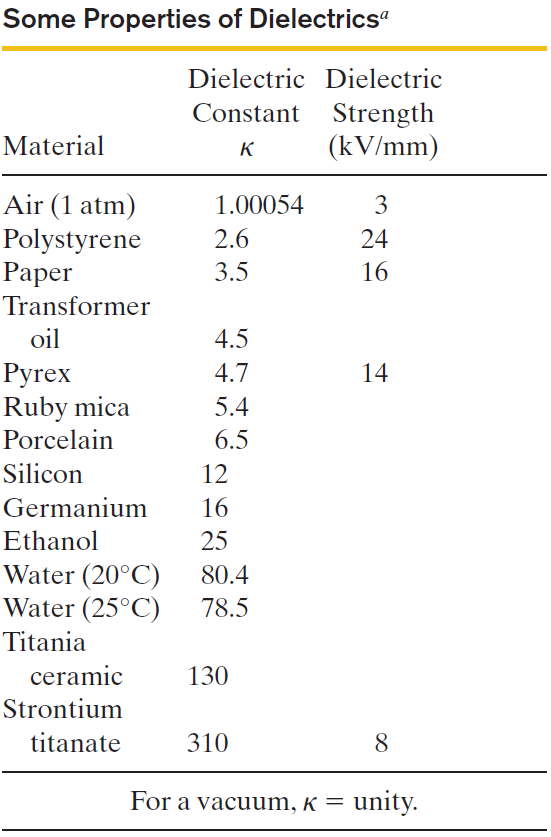
\includegraphics[width=4.7cm]{Physics2_PNGs/dielectrics.png}
			\caption*{}
			\label{fig:dielectrics.png}
		\end{wrapfigure}	
		If you fill the plates of a capacitor with a \textit{dielectric}, which is an insulating material, the capacitance increased by a numerical factor $\varepsilon_r$ ($\kappa$ in most textbooks) which is called \textbf{dielectric constant}. The dielectric constant of a vacuum is a unity by definition, since air is mostly empty space, it is just slightly greater than unity. \\
		If the plates of a capacitor (with distance $L$ between them) are filled with a dielectric then, the capacitance becomes:
		\[
			C = \varepsilon_r \varepsilon_0 L = \varepsilon_r C_{\text{vacuum}}
			\tag{5-25}
		\]
		By extension, in a region completely filled by a dielectric material of dielectric constant $\varepsilon_r$, all electrostatic equations containing the permittivity constant $\varepsilon_0$ are to be modified by replacing $\varepsilon_0$ with $\varepsilon_0 \varepsilon_r$\\ \\ \newpage
		For example:
		\[
			E = \frac{q}{4 \pi \varepsilon_r \varepsilon_0 r^2}
			\tag{Coulomb's Law for Point Charge, 5-26}
		\]
		\[
			E = \frac{\sigma}{\varepsilon_r \varepsilon_0}
			\tag{Electric Field just outside isolated conductor, 5-27}
		\]
		\[
			C = \frac{\varepsilon_0 \varepsilon_r A}{d}
			\tag{Parallel-Plate Capacitor, 5-28}
		\]
		\[
			C = \frac{2 \pi \varepsilon_0 \varepsilon_r L}{\ln (b/a)}
			\tag{Cylindrical Capacitor, 5-29}
		\]
		\[
			C = 4 \pi \varepsilon_0 \varepsilon_r \frac{ab}{b - a}
			\tag{Spherical Capacitor, 5-30}
		\]
		
		
		
		\subsection*{5.6 Dielectrics: An Atomic View}
		
		What happens at a molecular / atomic level? There are two possibilities, depending on the type of molecule:
		\begin{itemize}
			\item[1.]\textit{Polar dielectrics}: the molecules of some dielectrics have permanent electric dipole moment. In such materialsthe electric dipoles tend to line up with and external electric field.
			\item[2.]\textit{Nonpolar dielectrics}: regardless of whether they have permanent dipole moments, molecules acquire dipole moment by induction when placed in an external electric field, we can say that the external electric field tends to ``stretch'' the molecules.
		\end{itemize}
		
		\begin{figure}[!htbp]
			\centering
			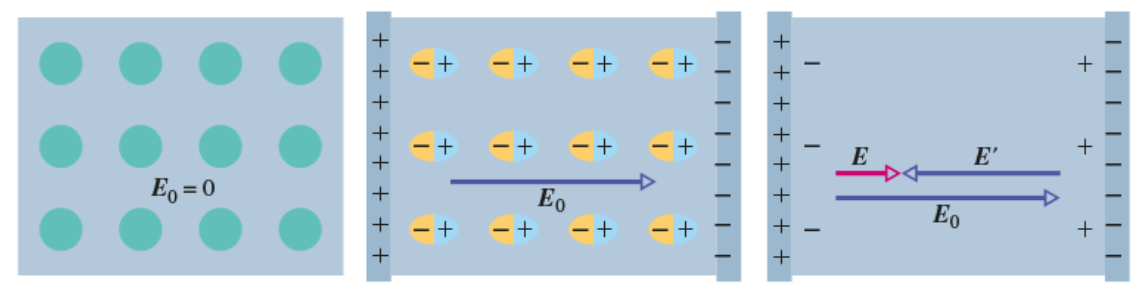
\includegraphics[width=10cm]{Physics2_PNGs/molecular-dipoles.png}
			\caption*{}
			\label{fig:molecular-dipoles.png}
		\end{figure}	
		When a nonpolar dielectric slab is placed in an external electric field (such as within a charged capacitor), the field causes a slight displacement of positive and negative charge centers within the material. This results in induced surface charges: \textit{positive} on one face and \textit{negative} on the opposite face, while the slab remains electrically neutral overall. These induced charges generate an internal electric field that opposes the applied field, reducing its net magnitude inside the dielectric. This behavior, observed in both polar and nonpolar dielectrics, weakens the effective electric field between capacitor plates, influencing capacitance. \\
		The resulting field
		\[
			\vec{E} = \vec{E_0} + \vec{E'} = \frac{\vec{E}}{\varepsilon_r}
		\]
		will always be less intense than $\vec{E_0}$ by a factor $\varepsilon_r$.
		
		
		
		\newpage
		
		\subsection*{5.7 Dielectric and Gauss' Law}
		
		\begin{wrapfigure}{r}{0.2\textwidth}
			\centering
			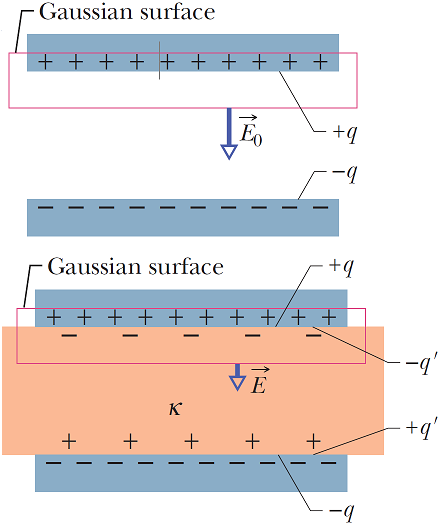
\includegraphics[width=5.5cm]{Physics2_PNGs/gaussian-surf-dielecs.png}
			\caption*{}
			\label{fig:gaussian-surf-dielecs.png}
		\end{wrapfigure}
		We generalize Gauss' Law in presence of any dielectric. \\
		We take a parallel-plate capacitor of plate area $A$ and we assume that the charge $q$ on the plates is the same. For a situation with no dielectric we can find the field $\vec{E_0}$ between the plates by enclosing the charge $+q$ with a Gaussian surface and then apply Gauss' Law. Letting $\vec{E_0}$ be the magnitude of the field:
		\[
			\varepsilon_0 \oint \vec{E} \cdot d\vec{A} = \varepsilon_0 E A = q
			\tag{5-31}
		\]
		or 
		\[
			E_0 = \frac{q}{\varepsilon_0 A}
			\tag{5-32}
		\]
		If we consider the case with a dielectric involved, we can find the electric field by using the same Gaussian surface, however the surface now encloses two different type of charge: the charge $+q$ on the plate and the charge $-q'$ on the top face of the \textit{dielectric}. The charge on the conducting plate is said to be \textit{free charge} because it can move if we change the potential of the plate, while the induced charge on the dielectric is not free charge since it cannot move from that surface. \\
		The net charge enclosed by the Gaussian surface is then $q - q'$, so Gauss Law' now gives
		\[
			\varepsilon_0 \oint \vec{E} \cdot d\vec{A} = \varepsilon_0 E A = q - q'
			\tag{5-33}
		\]
		or
		\[
			E = \frac{q - q'}{\varepsilon_0 A}
			\tag{5-34}
		\]
		The dielectric weakens the original field $E_0$ by a factor of $\varepsilon_r$, so we can write:
		\[
			E = \frac{E_0}{\varepsilon_r} = \frac{q}{\varepsilon_r \varepsilon_0 A}
			\tag{5-35}
		\]
		by comparing 5-34 and 5-35 we obtain that
		\[
			q - q' = \frac{q}{\varepsilon_r}
			\tag{5-36}
		\]
		By substituting for $q - q'$ into Eq. 5-31 we can write Gauss' law in the form:
		\begin{equation*}
			\varepsilon_0 \oint \varepsilon_r \vec{E} \cdot d\vec{A} = q
			\tag{Gauss' Law with Dielectric, 5-37}
		\end{equation*}
		By introducing the \textit{electric displacement} 
		$\vec{D} = \varepsilon_0 \varepsilon_0 \vec{E}$, and leaving the \textit{free charge} $q$ we can rewrite 5-37 in a more compact form:
		\[
			\oint \vec{D} \cdot d\vec{A} = q
			\tag{Gauss' Law with Dielectric, 5-38}
		\]
		
		
		\newpage
		
		
		\section*{6. Current and Resistance}
		
		
		\subsection*{6.1 Electric Current}
		
		\begin{wrapfigure}{r}{0.14\textwidth}
			\centering
			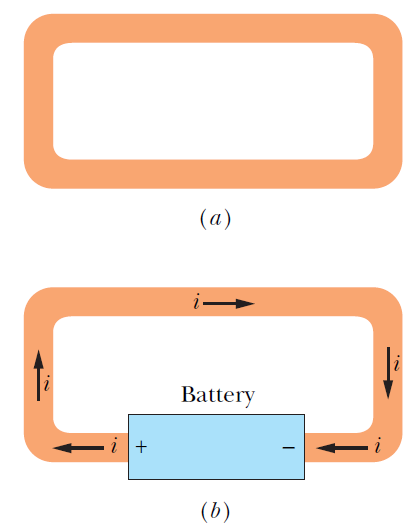
\includegraphics[width=4.5cm]{Physics2_PNGs/elec-current.png}
			\caption*{}
			\label{fig:elec-current.png}
		\end{wrapfigure}
		Although an electric current is a stream of moving charges, not every moving charges constitute an electric current. In order to have an electric current through any surface, there must be a net flow of charge. 
		Free electrons in a conductor have an effective speed of 
		$v_{\text{eff}} \approx 10^6 m/s$, but there's no \textit{net transport of charge}. \\
		Any isolated conducting loop, then has all same potential, thus no electric current. \\ 
		If we insert a battery in the loop, an \textit{Electric Field} is estabilished and acts on the material making up the loop, exerting forces onto the electrons, generating an \textit{electric current}. After an amount of time, the electron flow reaches a constant value and the current reaches a \textit{steady state}. \\
		If a charge $dq$ passes through an hypothetical plane in time $dt$, then the current $i$ going across that plane is defined as:
		\begin{equation*}
			i \triangleq \frac{dq}{dt}
			\tag{Definition of Current, 6-1}
		\end{equation*}
		We can find the charge that passes through the plane in a time interval
		($dq = i \, dt$) by integration:
		\[
			q = \int dq = \int_{0}^{t} i \, dt
			\tag{6-2}
		\]
		The current is the same in any cross section of said plane. \\ \\
		The SI unit for current is the \textit{coulomb per second}, or \textit{ampere} (A) which is an SI base unit:
		\begin{wrapfigure}{r}{0.14\textwidth}
			\centering
			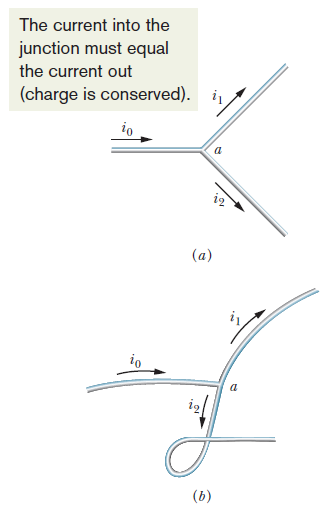
\includegraphics[width=5cm]{Physics2_PNGs/current-is-conserved.png}
			\caption*{}
			\label{fig:current-is-conserved.png}
		\end{wrapfigure}
		
		\[
			1 \, \text{ampere} = 1 \, \text{A} = 1 \, \text{coulomb per second}
			= 1 \, \text{C} / \text{s}
		\]
		
		\subsection*{6.1.1 Current is Conserved}
		

		Current, as defined on 6-1, is a scalar because both charge and time are scalars in the equation. If a current $i_0$ is split in two branches in a junction, since \textit{charge is conserved}, the magnitudes of the currents in the branches must add to match the current in the original conductor, therefore
		\[
			i_0 = i_1 + i_2
			\tag{First Law of Kirchhoff, 6-3}
		\]
		
		
		\subsection*{6.1.2 Directions of Currents}
		
		The direction of a current is the one in which the \textit{positive charges} would be carried, even if the effective \textbf{charge carriers} are \textit{negative} and move in the \textit{opposite direction}. \\
		In almost every situation, a positive charge in movement $+ \hat{x}$ has the same effect as the actual motion of negative charge in the opposite direction 
		$- \hat{x}$.
		
		
		
		\newpage
		
		\subsection*{6.2 Current Density}
		
		\begin{wrapfigure}{r}{0.14\textwidth}
			\centering
			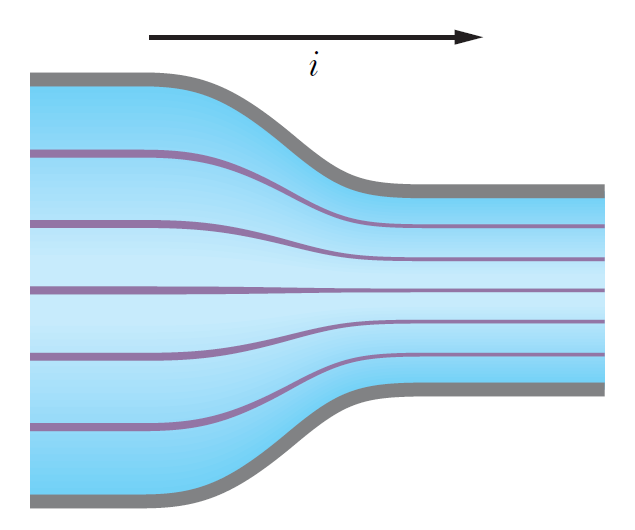
\includegraphics[width=4cm]{Physics2_PNGs/curr-density.png}
			\caption*{}
			\label{fig:curr-density.png}
		\end{wrapfigure}
		The flow of charge $i$ in a particolar point of a conductor can be described by the \textbf{current density} $\vec{J}$, which has same direction as the velocity of the moving charges if they are \textit{positive}, opposite direction if they are \textit{negative}. \\
		We can write the amount of current through the element as 
		$\vec{J} \cdot d\vec{A}$ where the area vector $d\vec{A}$ is perpendicular to the element. The total current through the surface is then:
		\begin{equation*}
			i = \int \vec{J} \cdot d\vec{A}
			\tag{6-4}
		\end{equation*}
		If the current is uniform across the surface and parallel to $d\vec{A}$, then $\vec{J}$ is also uniform and parallel. Eq. 6-4 becomes:
		\[
			i = \int J \, dA = J \int dA = JA
		\]
		therefore
		\[
			J = \frac{i}{A}
			\tag{6-5}
		\]
		where A is the total area of the surface. \\
		The SI unit for \textit{current density} is ampere per square meter (A/m$^2$).
		
		
		
		\subsection*{6.2.1 Drift Speed}
		
		\begin{wrapfigure}{r}{0.17\textwidth}
			\centering
			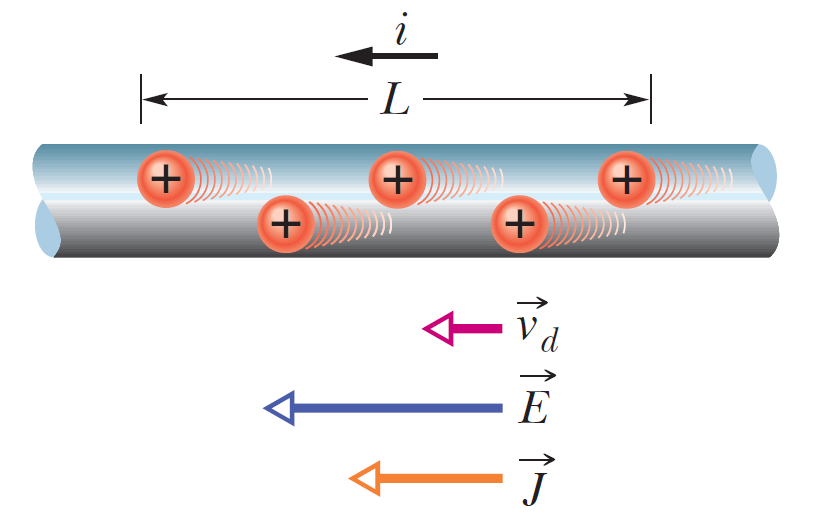
\includegraphics[width=5cm]{Physics2_PNGs/drift-speed.png}
			\caption*{}
			\label{fig:drift-speed.png}
		\end{wrapfigure}
		Without any kind of current, electrons move randomly with no net motion in any direction (with speed $v_{\text{eff}} \approx 10^6$ m$^2$/s). \\
		When a conductor does have a current instead, they tend to \textit{drift} with a \textbf{drift speed} $v_d \approx 10^{-5}$ m/s. \\
		
		We now relate the drift speed $v_d$ of the conduction electrons in a current through a wire to the magnitude $J$ of the current density in the wire. \\
		We take a wire of length $L$, with cross-section area $A$. The number of charge carriers in a length $L$ of the wire is $nAL$ (where $n$ is the number of \textit{carriers} per unit volume). The total charge of such carriers, each with charge $e$ is then:
		\[
			q = (nAL)e
		\]
		Since all the carriers move along the wire with speed $v_d$, this total charge moves across any section in a time interval:
		\[
			t = \frac{L}{v_d}
		\]
		Eq. 6-1 tells us that electric current is, by definition $i = q / t$, therefore:
		\[
			i = \frac{q}{t} = \frac{n A L e}{L / v_d} = n A e v_d
			\tag{6-6}
		\]
		by solving for $v_d$ and recalling Eq. 6-5 ($J = i / A$):
		\[
			v_d = \frac{i}{nAe} = \frac{J}{ne}
		\]
		or, extended to vector form:
		\begin{equation}
			\vec{J} = (ne) \vec{d}_d
			\tag{6-7}
		\end{equation}
		In which \textit{carrier charge density} ($ne$) SI unit is coulomb per cubic meter (C/m$^3$). \\
		$\vec{J}$ and $\vec{v_d}$ have same direction if $ne$ is \textit{positive}, opposite directions if $ne$ is \textit{negative}.
		
		
		
		\subsection*{6.3 Resistance and Resistivity}
		
		By applying a potential difference through a conductor, there will be a resultant electric current which will be different for any conductor. \\
		The characteristic of such conductor is called electrical \textbf{resistance}.
		\[
			R \triangleq \frac{V}{i}
			\tag{Definition of Electrical Resistance, \textbf{Ohm's Law}, 6-8}
		\]	
		The SI unit for resistance is the volt per ampere. This combination has a special name, which is the \textbf{ohm} (symbol $\Omega$). That is:
		\[
			1 \, \text{ohm} = 1 \, \Omega = 1 \text{volt per ampere} = 1 \, \text{V/A}
			\tag{6-9}
		\]
		A conductor whose function in a circuit is to provide a resistance is called \textbf{resistor} and in a diagram has symbol 
		\begin{circuitikz}
			\draw (0,0) to[R] (2,0);
		\end{circuitikz}
		, we can rewrite 6-8 as:
		\[
			i = \frac{V}{R} \quad \quad \quad \text{or} \quad \quad \quad V = iR
		\]
		
		
		
		\subsection*{6.3.1 Resistivity and Conductivity}
		
		\begin{wrapfigure}{r}{0.17\textwidth}
			\centering
			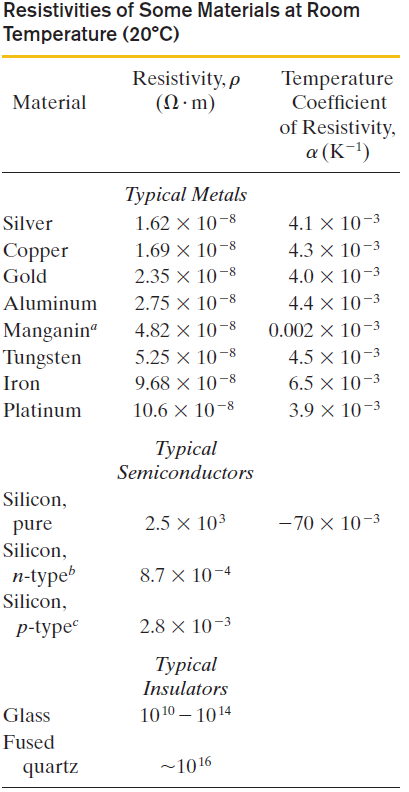
\includegraphics[width=5cm]{Physics2_PNGs/resistivities-table.png}
			\caption*{}
			\label{fig:resistivities-table.png}
		\end{wrapfigure}
		The potential $V$ through both ends of a resistor corresponds locally to an electric field $\vec{E}$. Instead of dealing with the current $i$ through the resistor, we deal with the current density $\vec{J}$ at the needed point. \\
		Instead of the resistance $R$, we deal with the \textbf{resistivity} $\rho$ oof the material:
		\[
			\rho \triangleq \frac{E}{J}
			\tag{Definition of Resistivity, 6-10}
		\]
		If we combine the SI units of $E$ and $J$, we get forr the unit of $\rho$ the \textit{ohm-meter} ($\Omega$ $\cdot$ m):
		\[
			\frac{\text{unit}(E)}{\text{unit}(J)} = \frac{\text{V/m}}{\text{A/m}^2}
			 = \frac{V}{A} m = \Omega \cdot \text{m}
		\]
		We can rewrite Eq. 6-10 in vector form as:
		\[
			\vec{E} = \rho \vec{J}
			\tag{Ohm's Law, 6-11}
		\]
		The \textbf{conductivity} $\sigma$, which is the reciprocal of the resistivity, is a measure of how ``well'' a material can conduct electricity:
		\[
			\sigma \triangleq \frac{1}{\rho}
			\tag{Definition of Conductivity, 6-12}
		\]
		Its SI unit is the reciprocal ohm-meter ($\Omega$ $\cdot$ m)$^{-1}$, which is also referred as \textit{mho per meter} ($\mho$/m) or \textit{Siemens per meter} (S/m). \\
		We can rewrite 6-11 as
		\[
			\vec{J} = \sigma \vec{E}
			\tag{6-13}
		\]
		
		
		
		\newpage
		
		\subsection*{6.3.2 Calculating Resistance from Resistivity}
		
		\begin{wrapfigure}{r}{0.22\textwidth}
			\centering
			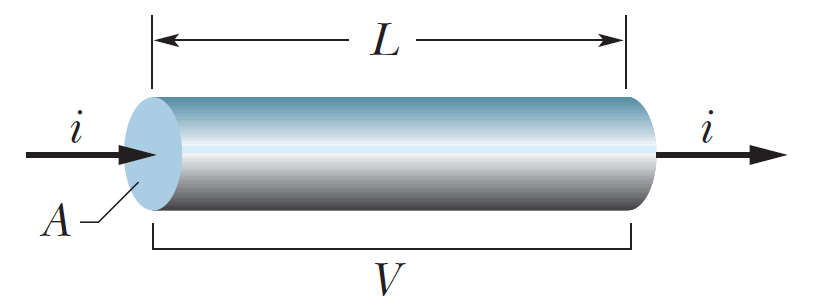
\includegraphics[width=6cm]{Physics2_PNGs/elec-wire-imm.png}
			\caption*{}
			\label{fig:elec-wire-imm.png}
		\end{wrapfigure}
		Resistance is a property of an object. \\
		Resistivity is a property of a material. \\\\
		Let $A$ be the cross-sectional area of a wire of length $L$, and let a potential difference $V$ exist between its ends.
		If the streamlines representing the current density are uniform throughout the wire, then the electric field and the current density will be constant at all points within the wire. \\
		We know that $E = V/L$ and $J = i/A$, by combining them:
		\[
			\rho = \frac{E}{J} = \frac{V/L}{i/A}
			\tag{6-14}
		\]
		However $V/i$ is the resistance $R$, this allows us to recast 6-14 as
		\[
			\rho = \frac{VA}{iL} \quad \rightarrow \quad  
			\rho = R \frac{A}{L} \quad \rightarrow \quad 
			R = \rho \frac{L}{A}
			\tag{6-15}
		\]
		Which can only be applied to homogeneous isotropi conductors of uniform cross section.
		
		
		
		\subsection*{6.3.3 Variation with Temperature}
		
		Resistivity vary with temperature, as most physical properties do. The relation between temperature and resistivity for most metal is fairly (almost) linear over a rather broad temperature range. \\
		We can write an empirical approximation:
		\[
			\rho - \rho_0 = \rho_0 \alpha ( T - T_0 )
			\tag{6-16}
		\]
		$T_0$ is a reference temperature (usually $T_0 = 293$K, room temperature) for which $\rho_0 = 1.69 \cdot 10^{-8}$. \\
		$\alpha$ is called \textit{temperature coefficient of resistivity}.
		
		
		
		
		\subsection*{6.4 Ohm's Law}
		
		A resistor is a conductor with a specified resistance, which is independent from any magnitude and direction (polarity) of the applied potential difference. \\ \\
		\textbf{Ohm's Law} is an assertion that the current through a device is \textit{always} directly proportional to the potential difference applied to the device. \\ \\
		Eventhough --for historical reason-- it's called law, not every device obeys it, for example, many semiconductors do \textit{not} obey Ohm's Law, since they do \textit{not} have constant resistance. \\\\
		A conducting \textbf{device} obeys Ohm's Law when the resistance of such device is independent of the magnitude polarity of the applied potential difference. 
		(if $\, \, V \propto i \quad$ and $\quad R = \frac{V}{i}$). \\ \\
		A conducting \textbf{material} obeys Ohm's Law when its resistivity is independent of the magnitude and direction of the applied electric field. (if $\, \, E \propto J \quad$ and $\quad \rho = \frac{E}{J}$).
		
		
		
		\subsection*{6.5 A Microscopic View of Ohm's Law}
		
		To find out why any particular material obeys Ohm's law, we must look into details at an atomic level. We consider only metals and we base the analysis on the free-electron model, in which we assume the conduction electrons can move freely troughout the volume of a sample, in a similar way to the molecules of a gas in a closed container. We also assume that the electrons do not collide with each other but do collide only with the atoms of the metal. \\
		After every collision the electron moves in a \textbf{random direction}. \\
		The motion of conducting electrons is an electric field $\vec{E}$, therefore a combination of the motion due to \textit{random collisions} and due to $\vec{E}$. If we consider all the free electrons, their drift speed is \textit{zero} and it only depends on the field $\vec{E}$.
		\\ 
		An electron of mass $m$, placed in an electric field of magnitude $E$ will experience an acceleration given by Newton's Second Law:
		\[
			a = \frac{F}{m} = \frac{eE}{m}
			\tag{6-17}
		\]
		In an average time $\tau$ between collisions, the average electron will acquire a drift speed $v_d = a \tau$. Then 6-17 becomes:
		\[
			v_d = a \tau = \frac{e E \tau}{m}
			\tag{6-18}			
		\]
		Combining this result with $\vec{J} = n e \vec{v_d}$, in magnitude form, yields:
		\[
			v_d = \frac{J}{n e} \quad \rightarrow \quad \frac{J}{n e} = \frac{e E \tau}{m}
			\tag{6-19}
		\]
		which, rewritten in terms of $E$:
		\[
			E = \biggl( \frac{m}{e^2 n \tau} \biggl) J
			\tag{6-20}
		\]
		comparing this with $\vec{E} = \rho \vec{J}$, in magnitude form leads to:
		\[
			\rho J = \biggl( \frac{m}{e^2 n \tau} \biggl) J \quad
			\rightarrow \quad \rho = \frac{m}{e^2 n \tau}
			\tag{6-21}
		\]
		We just showed that, for metals, their resistivity $\rho$ is a constant independent of the strength of the applied field $\vec{E}$. We can also assume that the number of electron $n$ is independent from the field, and $m$ and $e$ are constants. Also $\tau$ can be considered constant for this purpose, since the drift speed $v_d$ (caused by the field) is much smaller than the effective speed $v_{\text{eff}}$, therefore $\tau$ is hardly affected by the field. 
		
		
		
		\subsection*{6.6 Power in Electric Circuits}
		
		\begin{wrapfigure}{r}{0.16\textwidth}
			\centering
			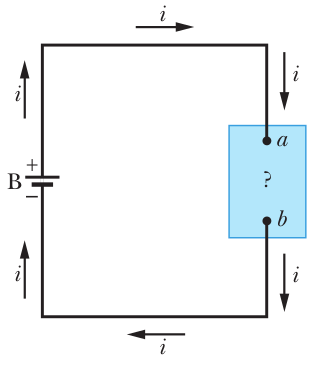
\includegraphics[width=4cm]{Physics2_PNGs/battery-circ.png}
			\caption*{}
			\label{fig:battery-circ.png}
		\end{wrapfigure}
		Battery B connecterd by wires, which we assume have negligible resistance to an unspecified conducting device (that might be a resistor, a motor, a storagge battery). The battery maintains a potential difference of magnitude $V$ across its own terminals and across the device terminals accordingly, with greater potential at terminal $a$ of the device than at $b$. \\
		A steady current $i$ is produced in the circuit, directed from $a$ to $b$. An amount of charge $dq$, that moves between those terminals in a time interval $dt$, is equal to $i \, dt$ ($dq = i \, dt$). This charges moves through a decrease in potential $V$ and thus its electric potential energy decreases in magnitude by an amount:
		\[
			dU = V \, dq = V \, i \, dt
			\tag{6-22}
		\] 
		The principle of conservation of energy tells us that the decrease in electric potential energy from $a$ to $b$ is accompanied by a transfer of energy to some other form. \\
		The power $P$ associated with that transfer is the rate of transfer $dU/dt$, which is given by:
		\[
			P = i \, V
			\tag{Rate of Electrical Energy Transfer, 6-23}
		\]
		which is also the amount of energy transferred from the battery to the device. \\
		The unit of power is the volt-ampere (V $\cdot$ A), and can be written as:
		\[
			1 \, \text{V} \cdot \text{A} = \biggl( \frac{\text{J}}{\text{C}} \biggl)
			  \biggl( \frac{\text{C}}{\text{s}} \biggl) = 1 \, \frac{\text{J}}{\text{s}}
			  = 1 \, \text{W} \, \, \, \text{[watt]}
		\]
		\\ \\
		In a resistor, or any device with resistance $R$, we can combine Eqs. $R = V / i$ and $P = iV$ to obtain:
		\[
			P = i^2 R
			\tag{Resistive Dissipation, 6-24}
		\]
		or
		\[
			P = \frac{V^2}{R}
			\tag{Resistive Dissipation, 6-25}
		\]
		Those two equation apply only on to the transfer of electric potential energy into thermal energy in a device \textit{with} resistance, while 6-23 ($P = iV$) applies to any kind of electrical energy transfer.
		
		
		
		\subsection*{6.7 Semiconductors}
		
		Semiconductors are materials with electrical conductivity between that of a conductor (like metals) and an insulator (like glass). This unique property allows them to control electrical current, making them essential in modern electronics. They are the backbone of devices like computers, smartphones, and solar cells.
		The most common material is pure silicon. Its resistivity can by controlled by adding a minute amount of ``impurity'' atoms in a process called \textit{doping}.
		
		\subsection*{6.8 Superconductors}
		
		Sure thing! Superconductors are materials that can conduct electricity with zero resistance when cooled below a certain critical temperature. This allows for incredibly efficient energy transfer and strong magnetic fields.
		
		
		
		
		\newpage
		
		\section*{7. Circuits}
		
		In order to make charge carriers flow through a resistor you must estabilish a potential difference $V$ between the ends of the device. We can achieve this by connecting a resistor to the ends of a capacitor plate, but a capacitor would discharge pretty quickly. \\
		To produce a steady flow, we need a ``charge pump'' a device that, by doing work on the charge carriers, maintains a constant potential difference $V$ between the terminals of the device. 
		\\ We call such device \textbf{emf device} and it is said to produce an \textbf{emf} \textbf{\calE}. \\
		A common emf device is the battery.
		
		
		
		\subsection*{7.1 Work, Energy and Emf}
		
		\begin{wrapfigure}{r}{0.20\textwidth}
			\centering
			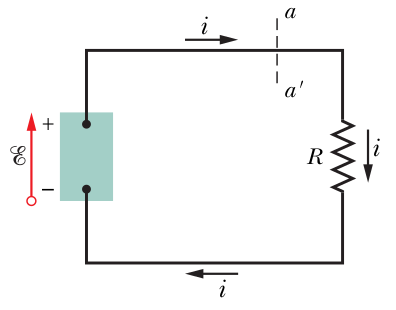
\includegraphics[width=5.5cm]{Physics2_PNGs/emf-device.png}
			\caption*{}
			\label{fig:emf-device.png}
		\end{wrapfigure}
		When an emf device is not connected to a circuit, no net flow is produced. However, when connected to a circuit, the internal chemistry of the device causes a net flow of positive charge carriers from the negative (--) to the positive (+) terminal of such device. \\
		Thus there must be some source of energy within the device, enabling it to do work on the charges and forcing them to move. \\
		If we analyze the circuit in figure, in any time $dt$ a charge $dq$ passes through any cross section of this circuit, such as $aa'$. This amount must enter the emf device at its low-potential end and leave at its high-potential end. \\
		The device must do an amount of work $dW$ on the charge $dq$ to force its movement.
		Therefore we define the emf \calE as:
		\[
			\calE = \frac{dW}{dq}
			\tag{Definition of \calE, 7-1}
		\]
		Its unit in term of SI is the Volt [V], or J/C.
		
		\subsection*{7.2 Calculating Current in a Single-Loop Circuit}
		
		\begin{wrapfigure}{r}{0.20\textwidth}
			\centering
			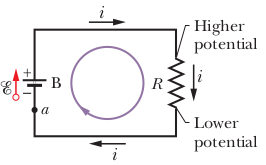
\includegraphics[width=5cm]{Physics2_PNGs/single-loop-circuit.png}
			\caption*{}
			\label{fig:single-loop-circuit.png}
		\end{wrapfigure}
		We now discuss two equivalent methods to calculate the current in a simple single-loop circuit. \\
		The circuit consists of a battery B with emf \calE, a resistor of resistance $R$ and two connecting wires, with negligible resistance.
		
		
		
		\subsection*{7.2.1 Energy Method}
		
		$P = i^2 R$ tells us that in a time interval $dt$ an amount of energy given by $i^2 R$ will appear in the resistor as thermal energy, which is said to be \textit{dissipated}. In the same interval a charge $dq = i \, dt$ will have moved through battery B, and the work that the battery will do on such charge is:
		\[
			dW = \calE \, dq = \calE i \, dt
		\]
		from the principle of conservation of energy, the work energy done must equal the thermal energy in the resistor:
		\[
			\calE i \, dt = i^2 R \, dt
		\]
		This gives us 
		\[
			\calE = i R
		\]
		By arranging for electric current $i$:
		\[
			i = \frac{\calE}{R}
			\tag{7-2}
		\]
		
		
		\subsection*{7.2.2 Potential Method}
		
		\textbf{Loop Rule}: The algebrahic sum of the charges in a potential encountered in a complete trasversal of any loop of a circuit must be \textit{zero}. \\\\
		This is often referred as \textit{Kirchhoff's loop rule}. \\
		Let's start at point $a$, whose potential is $V_a$ and ``walk'' clockwise around the circuit until we are back to $a$. Since the battery is ideal the potential difference between its terminals is \calE, when we pass through the battery to the high potential terminal, the change in potential is +\calE.	When passing through the resistor however, the potential changes according to $V = iR$ and must decrease since we are moving from the higher potential side of the resistor. Thus, we have change in potential $-iR$. \\
		We return to point $a$, aquiring potential $V_a$. Since we traversed the whole loop, the initial potential mus be equal to the final potential, therefore:
		\[
			V_a + \calE - iR = V_a \quad \rightarrow \quad \calE - iR = 0
		\]
		Solving for $i$ yields same result as earlier:
		\[
			i = \frac{\calE}{R}
		\]
		\textbf{Resistance Rule}: For a move through a resistance in the direction of the current, the change in potential is $-iR$; in the opposite direction $+iR$. \\\\
		\textbf{EMF Rule}: For a move through a emf device in the direction of the emf arrow, the change in potential is +\calE; -\calE otherwise.
		
		
		
		
		\subsection*{7.2.4 Internal Resistance}
		
		\begin{figure}[!htb]
			\centering
			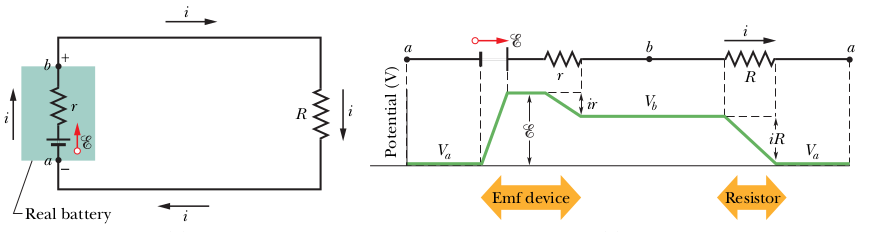
\includegraphics[width=10cm]{Physics2_PNGs/internal-resistance.png}
			\caption*{}
			\label{fig:internal-resistance.png}
		\end{figure}
		Any real battery has an internal resistance $r$ due to conductor materials' resistance (that's why is an unremovable feature). We can, however, draw the battery as if it could be separated into an ideal battery of emf \calE and a resistor $R$. By applying Kirchhoff Loop Rule:
		\[
			\calE - ir - iR = 0
			\tag{7-3}
		\]
		solving for current $i$ we find:
		\[
			i = \frac{\calE}{R + r}
			\tag{7-4}
		\]
		
		
		
		\subsection*{7.2.5 Resistances in Series}
		
		\begin{wrapfigure}{r}{0.17\textwidth}
			\centering
			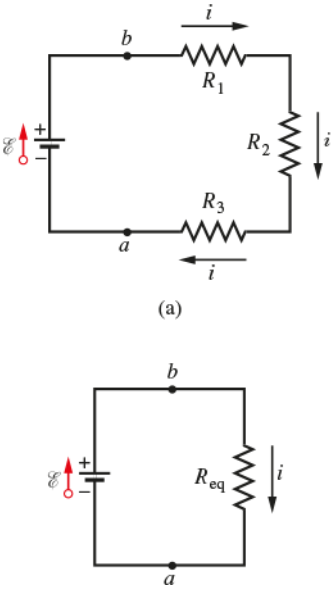
\includegraphics[width=4.5cm]{Physics2_PNGs/resistances-in-series.png}
			\caption*{}
			\label{fig:resistances-in-series.png}
		\end{wrapfigure}
		When a potential difference $V$ is applied across resistances connected in series, the resistances have identical currents $i$. The sum of the potential differences across the resistances is equal to the applied difference $V$. \\
		Resistance connected in series can be replaced by an equivalent $R_{eq}$ that has the same current $i$ and same \textit{total} potential difference $V$ as the actual resistance. \\\\
		We can derive an expression for $R_{eq}$ by using Kirchhoff's law:
		\[
			\calE - iR_1 - iR_2 - iR_3 = 0
		\]
		or, in terms of $i$:
		\[
			i = \frac{\calE}{R_1 + R_2 + R_3}
			\tag{7-5}
		\]
		By replacing $R_{eq} = R_1 + R_2 + R_3$:
		\[
			\calE - iR_{eq} = 0 \quad \quad \quad \text{or} \quad \quad \quad i = \frac{\calE}{R_{eq}}
			\tag{7-6}
		\]
		By extension to $n$ resistances:
		\[
			R_{eq} = \sum_{j=1}^{n} R_j
			\tag{\textit{n} Resistances in Series, 7-7}
		\]
		
		
		
		
		\subsection*{7.2.6 Grounding a Circuit}
		
		Grounding a circuit means connecting one part of the circuit to a reference point in the physical ground (earth) or to a conductive body that serves as a common return path. This reference point is called the "ground" which has potential $V = 0$ and has symbol   
		\begin{circuitikz} 
			\draw (0,-1) -- (0,-1) node[ground]{};  
		\end{circuitikz}  
		in diagrams. It provides a stable voltage level for the entire circuit.
		
		
		
		\subsection*{7.3 Multiloop Circuits}
		
		\begin{wrapfigure}{r}{0.17\textwidth}
			\centering
			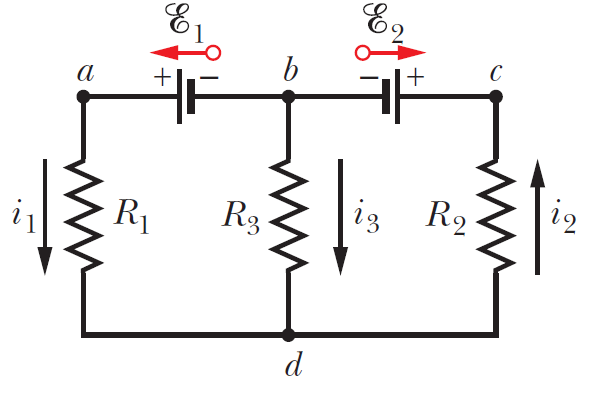
\includegraphics[width=4.5cm]{Physics2_PNGs/multi-loop.png}
			\caption*{}
			\label{fig:multi-loop.png}
		\end{wrapfigure}
		In figure we have a circuit containing two loops, with two \textit{junctions} $b$ and $d$ with three \textit{branches} connecting them. \\ \\
		\textbf{Junction Rule}: The sum of the currents entering any junction must be equal to the sum of the currents leaving that junction. \\
		Also called \textit{Kirchhoff's First Law}. \\ \\
		We consider the junction $d$, by applying Kirchoff's First Law:
		\[
			i_1 + i_3 = i_3
			\tag{7-8}
		\]
		Our basic tools to solve complex circuits are the \textit{loop rule} (based on conservation of energy) and the \textit{junction rule} (based on conservation of charge). \\
		To solve this circuit we apply the junction rule twice: \\
		If we traverse the left-hand loop in a counterclockwise direction from point $b$:
		\[
			\calE_1 - i_1 R_1 + i_3 R_3 = 0
			\tag{7-9}
		\]
		If we traverse the right-hand loop in a counterclockwise direction from point $b$: 
		\[
			- i_3 R_3 - i_2 R_2 - \calE_2 = 0
			\tag{7-10}
		\]
		We're now left with three equations (7-8, 7-9, 7-10) with three unknown currents, that can be solved in different ways.
		
		
		
		\subsection*{7.3.1 Resistances in Parallel}
 		
		\begin{wrapfigure}{r}{0.17\textwidth}
			\centering
			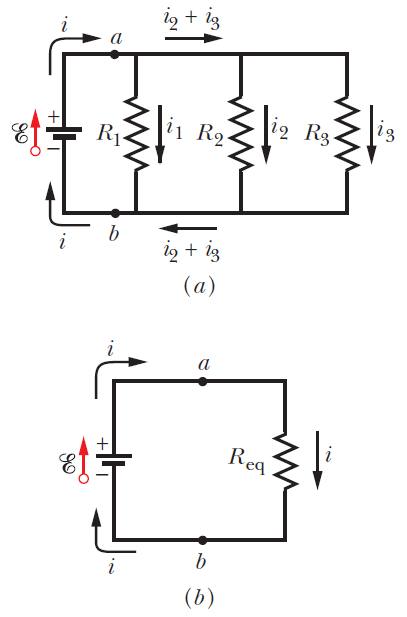
\includegraphics[width=4.5cm]{Physics2_PNGs/parallel-resistances.png}
			\caption*{}
			\label{fig:parallel-resistances.png}
		\end{wrapfigure}
		When a potential difference $V$ is applied across resistances connected in parallel, the resistances all have that same potential difference $V$. \\
		Resistances connected in parallel can be replaced with an equivalent resistance $R_{eq}$ that has the same potential difference $V$ and the same total current $i$ as the actual resistances.
		\\ \\
		We can derive an expression for $R_{eq}$ by evaluating the currents in the figure, first:
		\[
			i_1 = \frac{V}{R_1}, \quad i_2 = \frac{V}{R_2}, \quad i_3 = \frac{V}{R_3}
		\]
		where $V$ is the potential difference between $a$ and $b$. If we apply junction rule at point $a$ and then substitute the values for current:
		\[
			i = i_1 + i_2 + i_3 = V \, \biggl( \frac{1}{R_1} + \frac{1}{R_2} +
					                                    \frac{1}{R_3} \biggl)
			\tag{7-11}
		\]
		The equivalent resistance $R_{eq}$ is then:
		\[
			i = \frac{V}{R_{eq}} \quad \quad \text{or} \quad \quad
			\frac{1}{R_{eq}} = \frac{1}{R_1} + \frac{1}{R_2} + \frac{1}{R_3}
			\tag{7-12}
		\]
		Extending this result to $n$ parallel resistances:
		\[
			\frac{1}{R_{eq}} = \sum_{j=1}^{n} \frac{1}{R_j}
			\tag{\textit{n} Resistances in Parallel, 7-13}
		\]
		For the case of just \textit{two} resistances:
		\[
			R_{eq} = \frac{R_1 R_2}{R_1 + R_2}
			\tag{7-14}
		\]	
		\newpage
		
		\begin{table}[h]
			\centering
			\renewcommand{\arraystretch}{1.5} % Adjust row height
			\setlength{\tabcolsep}{5pt} % Reduce column spacing
			\begin{tabularx}{\textwidth}{|X|X|X|X|}
				\hline
				\multicolumn{2}{|c|}{\textbf{Resistors}} & \multicolumn{2}{c|}{\textbf{Capacitors}} \\
				\hline
				\textbf{Series} & \textbf{Parallel} & \textbf{Series} & \textbf{Parallel} \\
				\hline
				$ R_{\text{eq}} = \sum\limits_{j=1}^{n} R_j $ & 
				$ \frac{1}{R_{\text{eq}}} = \sum\limits_{j=1}^{n} \frac{1}{R_j} $ & 
				$ \frac{1}{C_{\text{eq}}} = \sum\limits_{j=1}^{n} \frac{1}{C_j} $ & 
				$ C_{\text{eq}} = \sum\limits_{j=1}^{n} C_j $ \\
				\hline
				Same current through all resistors & 
				Same potential difference across all resistors & 
				Same charge on all capacitors & 
				Same potential difference across all capacitors \\
				\hline
			\end{tabularx}
		\end{table}
		
		
		
		
		\subsection*{7.4 Ammeter and Voltmeter}
		 
		To measure current, the wire must be interrupted, and the ammeter must be inserted.
		Its resistance $R_A$ must be very small to avoid altering the circuit. \\\\
		To measure potential differences, the electrodes of the voltmeter must be connected without interrupting the circuit.
		Its resistance $R_V$​ must be very large to avoid altering the circuit.
		
		
		
		\subsection*{7.5 RC Circuits}
		
		\subsection*{7.5.1 Charging a Capacitor}
	
		\begin{wrapfigure}{r}{0.17\textwidth}
			\centering
			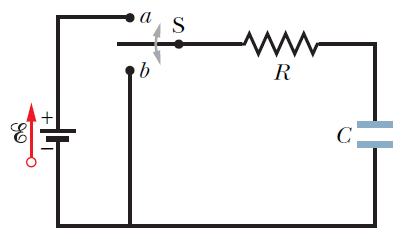
\includegraphics[width=4.5cm]{Physics2_PNGs/RC-circuit-png.png}
			\caption*{}
			\label{fig:RC-circuit-png.png}
		\end{wrapfigure}
		Capacitor of capacitance $C$, initially uncharged. To charge it we close switch S on point $a$. This completes an $RC$ \textit{series circuit} consisting of a capacitor, an ideal battery of emf \calE and a resistance $R$. \\
		The current starts to flow and increases the charges $q$ on the plates and the potential difference $V_C$ ($= q/C$) across the capacitor. When that potential difference equals the battery (which is here equal to emf \calE), the current is \textit{zero}. From $q = CV$ the \textit{equilibrium charge} on the then fully charged capacitor is equal to $C \calE$. \\
		We want to know how the charge $q(t)$ on the capacitor plates, the potential difference $V_C(t)$ across the capacitor and the current $i(t)$ vary with time. \\
		We apply loop rule traversing the circuit clockwise from the negative terminal of the battery:
		\[
			\calE - iR - \frac{q}{C} = 0
			\tag{7-15}
		\]
		We cannot solve this immediately since $i$ and $q$ are related:
		\[
			i = \frac{dq}{dt}
			\tag{7-16}
		\]
		By substituting 7-16 into 7-15:
		\[
			R \, \frac{dq}{dt} + \frac{q}{C} = \calE
			\tag{Charging Equation, 7-17}
		\]
		We solve this differential equation for $q$, by applying initial conditions $q = 0$ at $t = 0$ (since the capacitor is uncharged at the beginning). \\
		The solution is:
		\[
			q = C \calE ( 1 - e^{-t/RC})
			\tag{Charging a Capacitor, 7-18}
		\]
		
		\newpage
		\begin{wrapfigure}{r}{0.17\textwidth}
			\centering
			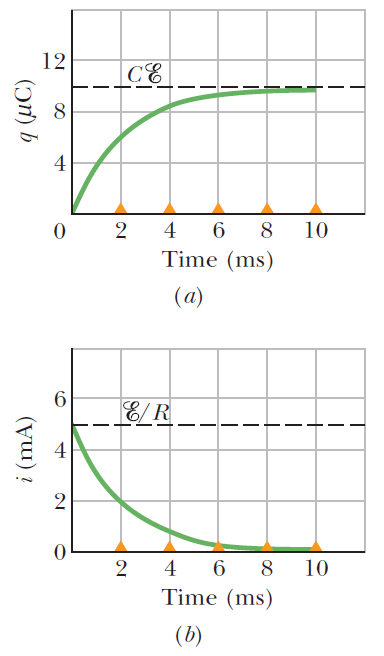
\includegraphics[width=4cm]{Physics2_PNGs/charging-capacitor-graph.png}
			\caption*{}
			\label{fig:charging-capacitor-graph.png}
		\end{wrapfigure}
		The derivative of $q(t)$ gives us the charging current $i(t)$:
		\[
			i = \frac{dq}{dt} = \biggl( \frac{\calE}{R} \biggl) e^{-t/RC}
			\tag{Charging a Capacitor, 7-19}
		\]
		A capacitor that is being charged initially acts like ordinary connecting wire relative to the charging current. A long time later, it acts like a broken wire.
		\\
		By combining $q = CV$ and Ec. 7-18 we find that the potential difference $V_C$ across the capacitor is:
		\[
			V_C = \frac{q}{C} = \calE (1 - e^{-t/RC} )
			\tag{Charging a Capacitor, 7-20}
		\]
		This tells us that $V_C = 0$ and $t = 0$ and therefore $V_C = \calE$ as the capacitor becomes fully charged at $t \rightarrow \infty$.
		
		
		
		\subsection*{7.5.2 Capacitive Time constant}
		
		We call the product $RC$ \textbf{capacitive time constant} of the circuit and is represented as;
		\[
			\tau = RC
			\tag{Capacitive Time Constant, 7-21}
		\]
		At time $t = \tau = RC$ the charge has increased from \textit{zero} to:
		\[
			q = C \calE (1 - e^{-1}) = 0.63 \calE
			\tag{7-22}
		\]
		In brief, during the first time constant $\tau$ the charge has increased from \textit{zero} to $63\%$.
		
		
		
		\subsection*{7.5.3 Discharging a Capacitor}
		
		At a time $t = 0$, we throw the switch S from $a$ to $b$. \\
		The differential equation describing $q(t)$ doesn't involve the battery now, $\calE = 0$. Thus:
		\[
			R \, \frac{dq}{dt} + \frac{q}{C} = \calE
			\tag{Discharging Equation, 7-23}
		\]
		This differential equation has solution:
		\[
			q = q_0 e^{-t/RC}
			\tag{Discharging a Capacitor, 7-24}
		\]
		or
		\[
			V = V_0 e^{-t/RC}
			\tag{7-25}
		\]
		where $q_0 = C V_0$ is the initial charge on the capacitor. \\
		This tells us that $q$ decreases exponentially with time at a rate $\tau = RC$. \\
		At time $t = \tau$ the capacitor charge reduces to $q_0 e^{-1}$, or about $37 \%$ of the initial value. \\
		Differentiating gives us the current $i(t)$:
		\[
			i = \frac{dq}{dt} = - \biggl( \frac{q_0}{RC} \biggl) e^{-t/RC}
			\tag{Discharging a Capacitor, 7-25}
		\]
		
		
		
		\newpage
		
		\section*{8. Magnetic Fields}
		
		
		
		
		
		
		
			
		
		
	
	
	

	\end{document}